\documentclass[a4paper,12pt]{article}
\usepackage{amsfonts}
\usepackage{graphicx}
% \usepackage[utf8]{inputenc}
% \usepackage[english]{babel}

%hyperlinks
\usepackage{hyperref}
\usepackage{float}

% Citations
% \usepackage[
% backend=biber,
% style=alphabetic,
% sorting=ynt
% ]{biblatex}
% \addbibresource{./section-references/citation}

% \usepackage{biblatex}

% \renewcommand\bibname{References}

\usepackage{fvextra}
\DefineVerbatimEnvironment{refs}
{Verbatim}
{fontfamily=\rmdefault,breaklines,breaksymbolleft={}}



\begin{document}

    %%%%%%%%%%%%%%%%%%%%%
    % Settings %
    %%%%%%%%%%%%%%%%%%%%%

    % Space before-after equations %
    % \setlength{\abovedisplayskip}{6pt}
    % \setlength{\belowdisplayskip}{6pt}
    \setlength{\abovedisplayshortskip}{6pt}
    \setlength{\belowdisplayshortskip}{24pt}
    
    % Space between paragraphs %
    \setlength\parskip{0.5\baselineskip}

    % New environment for definitions
    \newcounter{definition}[section]
    \newenvironment{definition}[1][]{\refstepcounter{definition}\par\medskip
        \noindent \textbf{Definition #1:} \rmfamily}{\medskip}

    % New environment for examples
    \newcounter{example}[section]
    \newenvironment{example}[1][]{\refstepcounter{example}\par\medskip
        \noindent \textbf{Example~\theexample. #1} \rmfamily}{\medskip}

    
    %%%%%%%%%%%%%%%%%%%%%
    % Document %
    %%%%%%%%%%%%%%%%%%%%%
    \title{Thesis}
    \author{Daniel Travaglia}
    \date{\today}
    \maketitle

    \pagebreak

    % table of contents here
    % \tableofcontents

    \pagebreak
    
    % Let's divide the document into sections (i.e. chapters)
    \section{A gentle introduction to credit risk}

    This section aims to give an overview of the topic that is at the heart of this paper: \textbf{credit risk}. 
    Rather than jumping straight into formal definitions, which might create difficulties in grasping with the content, 
    the reader will be first provided with real-life examples characterized by the presence of such risk. 
    Moving on, some formal definitions will be given along with a description of the agents that usually take upon 
    this risk and how they act to assess it and quantify it and finally take proper actions to mitigate it. 
    To conclude, the chapter ends with an introduction to credit risk modelling, 
    a topic that will be further explored later in the empirical analysis

    \subsection[]{Introduction} 
    
    In a recently published online course on credit analysis [Beeson, 2019], 
    the author provides a few real-life situations that occur daily and where it is possible to encounter credit risks. 
    The following examples are based on those situations and might serve as a great starting point to understand the topic. 
    
    \begin{example}
        Imagine yourself receiving a call from one of your friends that you have not heard for quite a while. 
        You can hear from his voice that he is really upset, and apparently, the reason for this is that 
        he has to pay a fine by the end of the day to avoid an additional charge, but he does not have the money 
        to pay at that moment. He tells you that the reason for this is that he had to cover fo huge expenses lately 
        and he still has not received his monthly salary. Given that, he then asks you, whether you would be kind enough to lend 
        him the money, promising to repay you as soon as he receives his pay. What would you do? Would you lend him the money? 
    \end{example} 

    \begin{example}
        Imagine to be in the same situation as above, but instead of simply being one of your friends, 
        the requestor is one of your colleagues at work? Would you do it in this case? Would it make a 
        difference if it was someone you knew well, for instance, the colleague you always work with? 
    \end{example}

    \begin{example}
        Imagine now the request to change, and instead of asking for a large sum, your colleague asks you to lend
        him money for a pizza without mentioning you when and how is going to pay you back. Would this make a difference 
        in your evaluation on whether to lend the money or not?
    \end{example}

 
    Although representing a very simplistic situation concerning what usually financial institutions have to deal with 
    when they need to evaluate whether to grant the credit or not, the questions that need to be answered could be equivalent: 

        \begin{enumerate} \item Who is borrowing? \item How much are they borrowing? \item When will the debt be fully repaid? \item How much is there for me (either as an individual or an institution)?
        \end{enumerate}
    
    Considering the last example, imagine instead that your colleague promises you to pay back the week after and on top of that,
    he is willing to take you out for lunch. This time, what you get back is more than what you lent. 
    In financial terms, this is also known as \textit{interest rate}. On the other hand, imagine he gives you his watch to keep 
    until he pays you back to make the lending much safer for you. The watch in this case represents a \textit{collateral} 
    (or a \textit{security}).

    The procedure just introduced is usually called "\textbf{credit analysis}". According to [Beeson, 2019], 
    the latter can be defined as: "\textit{the process through which the lender elaborates if he believes the counterparty is going to honour its obligations or not}". 
    Ultimately, this determines whether or not the agent will enter in that contract, 
    along with the relative risk associated with it, or more precisely, the \textbf{credit risk} [BIS, 2019].

    \subsubsection{Credit risk}

    It is possible to find many definitions of \textit{credit risk} around.
    \href{https://www.investopedia.com/}{Investopedia} provides us with the right one in this context:
 
        \begin{definition}[(Credit Risk)] \textit{the risk that a lender has to take into account due to the uncertainty related to the borrower either failing to repay a loan or to meet its obligations.} [Labarre, 2019]
        \end{definition}

    In simple terms, this definition suggests that the lender should consider the possibility that a borrower 
    will not be able to pay back the principal and the interest rate according to the initial contractual agreement. 
    The party granting the credit should then quantify this probability and based on the result, 
    charge a coupon rate (i.e. interest rate) to protect itself against this risk. 
    The methods to derive the likelihood a counterparty won't be able to meet the contractual agreements are 
    part of the broad area of \textbf{Credit Risk Modelling} [Bluhm, 2016]  
    which will be at the heart of the empirical analysis, and for this reason, it is introduced later in the paper. 
        
    Ultimately, in the context of credit risk there are at least 3 additional points [Labarre, 2019] 
    worth to mention which should also be considered as key takeaways from this introductory chapter:  
        \begin{enumerate} \item \textbf{Credit risk in every financial transaction}: although most of the times it might come naturally to associate this type of risk to transactions that occur exclusively between a party and a financial institution (e.g. mortgages, loans, credit cards, etc...), there are also situations where credit risk can be perceived between private parties (e.g. between companies and individuals: paying invoices, insurance coverage, etc..)   \item \textbf{Risk assessment}: before granting new credit (as often it is the case in the business world), the bank undergoes an assessment of the borrower takes into consideration his credit history, the capabilities to repay, the capital available, the loan's conditions and associated collateral. Such evaluation has the final goal of providing an accurate prior estimate of the credit risk, which will eventually tell whether the client should get or not the obligations, with an increasing interest rate for those who are perceived as riskier. In the case of bonds, this assessment is done by credit-rating agencies that assign a triple-A (i.e \textit{AAA}) for low-risk investments, all the way down to \textit{C} for high-risk investments. Note that, although this process is almost exclusively conducted for bond products, the dataset used in the empirical analysis provides the same ratings for loans, perhaps as a result of internal procedures to assess credit risk. \item \textbf{Credit risk vs. other risks}: so far it was assumed that the risk associated with the lending was purely driven by the borrower characteristics. However, in a typical lending transaction, usually, there are other types of risks kicking in: market risks (e.g. economic conditions, FX rates), country-specific risks (e.g. OECD country, emerging-markets country, etc..), operational risk, issuer risk, and so on... To keep things simple, and given the nature of the data for the empirical analysis, although it might represent a far too simplistic assumption, we will stick with it and only deal with a particular type of credit risk: the \textit{CCR (Counterparty Credit Risk)}       
        \end{enumerate}
        
    \subsubsection{CCR - Counterparty Credit Risk}

    According to \href{https://www.bis.org/}{BIS - Bank for International Settlments}, \textit{CCR (Counterparty Credit Risk)} can be defined as:
    
        \begin{definition}[(Counterparty Credit Risk)] \textit{the measure of the \textbf{likelihood} that the counterparty to a transaction \textbf{might default} before meeting the contractual obligation.} [BIS CCR, 2019]
        \end{definition}

        There is a subtle but fundamental difference between the two types of risk introduced above: 
        when assessing the "credit risk" in general, the lender takes into account the chance that the 
        borrower might not be able to fully repay the lender according to the contractual obligations, 
        but do not exclude that the counterparty might cover for the remaining part in the future either. 
        Hence, the bank is exposed (in terms of risk) only to the portion of the money lent that is perceived as being at risk. 
        
        On the other hand, the lender might also consider the possibility that the counterparty defaults on this loan 
        with the inability to bear the debt neither in the present nor in the future. 
        In such a context, the lender not only has to evaluate the risk associated with the loan, 
        but it also has to take into account the risk associated with the counterparty itself. 
        In conclusion, if such an event occurs, and the pool of transactions with the counterparty has a positive economic value, 
        the result would be an economic loss for the lender. 

        As a last note, CCR is usually characterized by the bilateral risk of loss (i.e. either one of the parties involved in the transaction might default). 
        Bilateral exposures usually factor in the uncertainty related to market movements, as part of the value of the transaction is driven by the underlying market value [BIS CCR, 2019].
        Nevertheless, during the empirical analysis, we will assume unilateral exposures: 
        the lender is the only one party to be exposed to the risk of the counterparty to default.


    \pagebreak
    \section{Basel Regulatory Framework}

    \subsection{Introduction}
    This section aims to introduce the key regulatory framework in the context of credit risk and more specifically, 
    counterparty credit risk: the Basel Accord. With a walk-through in history, 
    the objective is to make the reader aware of the reasons why lenders and companies have become increasingly regulated from this standpoint.
    \newline\newline
    % Reference
    \textbf{Note}: the content provided in this chapter is for the most part based on the information extracted from [Sukhy, 2020] and [Mario, 2020]

    \subsection{Reasons for a more comprehensive framework to credit risk management}
    
    The needs for a more comprehensive and better approach to risk management, 
    particularly for counterparty credit risk, has emerged quite significantly 
    after the financial crisis of 2007-2009. Since then, regulators have sharpened 
    their existing frameworks and applied more stringent controls to 
    the stability of financial institutions. On this line of reasoning, 
    this section provides an overview of how regulatory requirements in 
    the context of counterparty credit risk have evolved, with a focus on the 
    key regulatory framework in this environment: \textbf{The Basel Accords} [Chen, 2019]

    After the well-known and aforementioned 2007-2009 financial crisis event, 
    there has been an unprecedented revision of the global framework regulating 
    the financial sector, culminating in what is known today as the \textbf{Basel III} regulatory framework.
    Before reaching this result, the banking sector has experienced a 
    relevant number of systemic crisis usually driven by various factors, 
    including the miscalculation of risk, represented by inadequate capital levels 
    to carry out their business. Each of this crisis brought some contributions and 
    changes to the previous framework, adding up to the first version, 
    which consisted of 30 pages, more than 1500 pages of guidelines 
    relating to the supervision of daily banking activities. 

    \subsection{Reasons for an independent Committee}
    Why was the Basel Committee ever needed? 
    To answer this question, it is necessary to go back to 1970s, 
    when the Herstatt Bank collapsed and was put under liquidation due to 
    enormous trades on the foreign exchange market that did not go as planned. 
    The license was withdrawn in 1974, as losses have reached an amount equal to 
    10 times the liquidity of the bank. However, there is more to the story: 
    US counterparties engaging in multiple transactions with Hersatt Bank released 
    "Deutschmark" in exchange of dollars.
    These lenders did never see their money, essentially because of time differences: 
    the US was still in morning trades when the bank was revoked its license. 
    Although this is purely related to FX activities, and consequently involves 
    also FX and market risk, this event highlighted the necessity to create a 
    central forum for banking supervision concerning matters related also to 
    other types of risks, such as "credit risk". To enhance the financial stability 
    and quality of banking supervision, in 1974 multiple central banks gave rise to a 
    centralized committee which later on took the name of "Basel Committee on 
    Banking Supervision". The latter expanded quite significantly and as of now, 
    it includes 45 central banks worldwide.

    \subsection{Basel Frameworks}

    The need for a regulatory framework for risk management was further strengthened 
    during the 70s-80s period, when the surge in debt in the Latin American countries, 
    combined with the rise of interest rates in the US and Europe, led the way to a 
    series of critical debt restructuring efforts for many countries worldwide. 
    The need for a clearer and comprehensive framework for the banking sector 
    forced the Basel committee to issue guidelines on weighted approach to 
    risk management. 
    Such need was satisfied with the release of the \textbf{Basel 1} [BIS Basel I, 2004] 
    framework in 1988 when for the first time in history, 
    banks were required to weigh the capital they held against the credit risk they took. 
    
    \subsubsection[]{Basel 1}
    In 1988, the first regulatory framework, which later took the name of "Basel I", 
    was released by the Basel Committee. The latter had the objective of setting up 
    common international and shared regulations on capital adequacy supervision. 
    The relevant aspects of the regulation are summarized in the following points:
    
    \begin{itemize}
        \item Credit institutions are required to classify assets into 5 different categories based on their underlying risk: from 0\% for most secured assets (e.g. cash) to 100\% for low-quality assets (e.g. private sector debt). These assets are also identified as \textbf{RWA}" (risk-weighted assets).
        \item Definition of the so-called \textbf{Minimum Capital Requirement}: the minimum ratio of capital to risk-weighted assets (RWA). The threshold was initially set at \textit{8\%}, equally spread between most absorbing assets (i.e. \textbf{Tier-1 Capital}: examples are equity and retained earnings) and supplementary assets (\textbf{Tier-2 Capital}: examples are evaluated assets and subordinated debt). The latter includes assets that are more difficult to liquidate, and therefore less secure. This level was introduced to ensure that financial institutions had enough standalone capabilities to absorb potential losses resulting from defaulting clients. [Nickolas, 2020]
    \end{itemize}
    
    Despite the effort, the first Basel Regulation had some shortcomings. 
    These were mainly related to 3 factors: 
    the duration of the service, 
    the market risk and, most importantly, 
    the counterparty risk. 
    The introduction of amendments helped in assessing some of these issues
    (such as the Market Risk Amendment). 
    Nevertheless, the complexity introduced by some financial products 
    (Credit default swaps, Complex derivatives, etc..) was drastically incrementing 
    the risk taken by financial institutions. 
    This situation required further adjustments with the regulation and 
    shined a light on the ever-increasing importance of accurate methodologies 
    to assess exposures to risk. 
    
    \subsubsection[]{Basel 2}
    The proposal for a replacement of the previous accord (i.e. Basel I) came in 1999 
    and was finally released in 2004 with the name \textbf{Basel II}. [BIS Basel II, 2004]
    This comprised some of the previously mentioned and much-needed adjustments, 
    which are summarized here:

    \begin{enumerate}
        \item \textbf{Minimum capital requirements} [BIS Basel III, 2010]: it was developed and expanded and a new capital tier (i.e. \textbf{Tier-3}) was introduced to cover also for the market risk.
        \item \textbf{Market discipline}: financial institutions are obliged to periodically disclose information on their risk exposures to enable much more informed decisions and constant monitoring.
        \item \textbf{Supervisory review}: providing clear guidances on periodic assessments of an institution's capital adequacy and in case of capital pressure, it granted intervention powers
    \end{enumerate}

    Despite the efforts to bring more stability, 
    the accord required time and effort before it was released. 
    Most financial institutions had already started taking 
    full advantage of the subprime mortgages - lending money to low credit profile - 
    given their higher expected returns. 
    Moreover, these institutions entered the financial crisis with too much leverage 
    supported by the later favourable economic conditions, despite the regulatory 
    environment that was set in place with Basel II. These events were part of a 
    much broader series of dysfunctionality (e.g. poor governance, bad risk management, 
    a combination of excessive credit growth and credit risk mispricing) 
    that served as key lessons for the Basel Committee to bring substantial updates 
    to the baseline framework. Eventually, the Committee agreed to design a reform 
    package to outline new ways of handling credit and liquidity risk.

    \subsubsection[]{Basel 3}
    The agreement culminated with the publication in 2010 of what is today known 
    as the \textbf{Basel III} framework [BIS Basel III, 2010]. The aim was to improve on top of the 3 
    pillars of the previous accord and extend them to also other areas. 
    The key changes can be summarized in the following points:
    
        \begin{enumerate} 
            \item \textbf{Capital conservation buffer} [Kagan 2020]: part of the common equity that, if ever breached, restricts payouts (e.g. dividends) to be used to meet the minimum common equity requirements. 
            \item \textbf{New leverage ratio} [Hayes, 2020]: based on loss-absorbing capital and total institution's assets and takes into account also off-balance sheet exposures (regardless of RWA). 
            \item \textbf{Liquidity Coverage Ratio (LCR)} [Murphy, 2020]: a minimum short-term liquidity ratio to provide banks with enough liquidity to cover for at least 30-days stress period. 
            \item \textbf{Net Stable Funding Ratio (NSFR)} [BIS NSFR, 2014]: a minimum long-term liquidity ratio to address maturity mismatches over the balance sheet.
        \end{enumerate}

    The Basel Committee realized that the approach of "one fits all" 
    is hard to meet the expectations outlined in the framework. 
    For this reason, it started a series of reform to condition the 
    requirements on the institutions' size, complexity and systematic importance. 
    This culminated in a series of on-going reform packages that are still happening 
    today and should be published under the name of \textbf{Basel IV}.
    \newline

    % CONCLUSION -> FROM REGULATION -> TO HIRING IN CREDIT RISK -> RISK MODELLING -> CLOSE THE GAP WITH INFORMATION -> ASYMMETRIC IMPERFECTIONS
    
    \pagebreak
    \section{Credit Risk - Empirical Analysis}

    The objective of this section is to give a high-level overview of the methodologies 
    that the financial industry usually adopt to forecast credit losses and later leverage 
    the data available to develop a machine-learning approach and estimate the probability 
    that a counterparty will default on its obligation.

    \subsection[]{Credit risk modeling}
    
        \subsubsection{Introduction}
        The motivations for a financial institution to develop credit risk models are much due to 
        regulatory requirements. However, as highlighted in [Bluhm, 2016], 
        other reasons explain the importance of internal credit risk modelling. 
        To better understand this, let us provide a simplified, but not too unrealistic 
        example based on the example provided in [Bluhm, 2016]: 
   
    \begin{example}

        Imagine a bank is asked from a major tech company to provide a very huge loan in the size of \$5B. 
        As already discussed, a credit analyst, (who for ease the example we will call Ben) will have to 
        go through the request and see whether it is the case to grant or not this loan based on the 
        information that he can gather. Let us assume that Ben already knows that the CEO of this company 
        has a great friendly relationship with the CFO of the bank, and, from recent studies, 
        he discovers that the specific sector of the company has recently experienced
        a steady drop in sales and the bank-internal rating system suggests this company 
        is on its way down to a sub-investment grade (i.e. classified as a risky investment). 
        What should Ben do in this situation? Usually, the analyst has 2 options at this stage:

        \begin{enumerate} \item \textit{Reject} the deal based on the information he gathered on the company and the relative market \item \textit{Accept} the deal BUT, protect the bank against potential losses thanks to \textbf{credit risk management instruments} (such as credit derivatives) and transfer the risk to a third-party in exchange of a fee. [Chen, 2019]
        \end{enumerate}

    \end{example}

    Hence, financial institutions have also a way out: as individuals would do through health insurance, 
    banks can protect themselves from the underlying exposures to risk when lending to particularly risky clients. 
    In particular, banks had already designed ways to get loan insurance in the past and usually comprises 
    the whole bank's credit risk portfolio, and not only some critical positions. 
    This brings directly to what in [Bluhm, 2016]  is perceived as the building block of 
    credit risk modelling within a financial institution: the \textbf{expected loss}.

    \subsubsection{Expected Loss}
    For banks to protect against this risk, they would like to know the \textit{cost} 
    that arises from a particular client (a group of clients when dealing with a portfolio of loans) 
    before granting the loan, so that they can charge a \textit{premium} on the interest rate accordingly 
    and add up to a reserve (also called \textit{expected loss reserve}) to cover for potential losses 
    due to defaulting loans.
    In this context, the bank is interested to know, \textit{on average}, 
    the potential loss that might occur when lending money to a client.
    This value is called \textbf{Expected Loss} and it is characterized 
    by the 3 pillars of credit risk modelling [Chatterjee, 2015]:

        \begin{enumerate} \item \textbf{Probability of Default (PD)}: the \textit{likelihood} of a default in a defined time-horizon associated to a client. Note however that this is a general definition that may vary depending on the method used to estimate such probability. For instance, under the Basel II IRB framework, the PD per rating rate is defined as the average percentage of obligators that will default over one year (i.e. the time-horizon specified in the regulation for each asset class). \item \textbf{Exposure At Default (EAD)}: \textit{estimated outstanding amount} given that a client defaulted \item \textbf{Loss Given Default (LGD)}: \textit{proportion of EAD} that is expected not to be recovered in case of default.
        \end{enumerate}

    To be mathematically rigorous, the model describing the expected loss is defined on top of a probability space ($\Omega,\Phi,\mathcal{P}$), where $\Omega$ consists of the \textit{sample space} defining all the possible events, 
    $\Phi$ is the \textit{$\sigma$-Algebra} containing all the measurable events of the sample space (such as the information on whether an obligator default or not) and lastly, 
    $\mathcal{P}$, the probability space, which attaches a probability to each measurable event.

    If we declare $\textbf{\textit{D}}_{i}$ as the event that the client '\textit{i}' defaults within a time-horizon and $\mathcal{P}(D_{i})$ as the probability associated to this event, then 
    the loss related to the obligator can be then defined as:
    
    \begin{equation}
        L_{i}=I*EAD_{i}*LGD_{i} \quad\mathrm{with}\quad  I = \mathrm{\textbf{1}}_{D_{i}}, \quad\mathcal{P}(D_{i}) = PD_{i}
    \end{equation}
    where $I$ is equal to the \textit{indicator function} of the underlying event \textit{D}. The variable takes value 1 when the 
    event occur (i.e. default) and 0 when it does not occur. Note that this is a Bernoulli R.V., and as such, the expectation is equal to the probability of the event to occur. In other words, it is equal to the \textit{Probability of Default (PD)}. 
    Before laying down the formula of \textit{Expected Loss}, is necessary to list down some assumptions ([Chatterjee, 2015], [Bluhm, 2016] ):
    
    \begin{enumerate}
        \item To keep things simple, we will assume that the 3 constituents of the loss formula (i.e. PD, EAD, LGD) are independent among each other. Despite being a more than questionable statement and far from being true in general, this setting will allow us to state the most simple formula for the \textit{Expected loss}.
        \item To be able to simply define the expected loss over the whole portfolio of obligations, we also assume the joint distribution to be composed of independent and identically distributed R.V., each describing the expected loss of a specific obligator (\textit{i}).
    \end{enumerate}

    The formula of the expected loss of an obligator now comes very naturally as it is simply the expectation of the loss function defined above:

        \begin{equation} E[L_{i}]=\mathcal{P}(D_{i})*EAD_{i}*LGD_{i}
        \end{equation}
    
    where $\mathcal{P}(D_{i})$ represents the expectation of $I$.

    At this point, it is possible to identify the expected loss of a portfolio as the proportion of obligators that might default over a time-horizon,
    multiplied by the expected portion of the total expected exposures that is assumed not to be recovered if the default event occurs. More formally:

        \begin{equation} E[L_{P}]=\sum_{i=1}^{N} \mathcal{P}(D_{i})*EAD_{i}*LGD_{i}
        \end{equation}

    \subsubsection{Unexpected Loss}
    Note that the formula to calculate the expected losses aims at measuring the \textbf{expected} 
    proportion of losses due to defaulting obligators based on historical default experiences, 
    but it does not consider the \textbf{unexpected} losses that might come up as a deviation 
    from the average experienced losses of the past. [Bluhm, 2016] . 
    The capital held to sustain losses should then consider both, and for the sake of completeness of this chapter, 
    the formula will be provided here:

    \begin{equation}
        UL_{P}=\sum_{i=1}^{N} \sigma_{i}*\varphi_{i}
    \end{equation}
    where $\sigma_{i}$ is the individual standard deviation of credit losses for the obligator \textit{i}, while $\varphi_{i}$ indicates the correlation between the credit losses of individual \textit{i} and all the other obligators in the portfolio.

    After this brief parenthesis, let us go back to one of the key constituents of expected loss, the
    \textbf{probability of default}.

    \subsubsection{Probability of Default}
    \label{sec:calibration}

    Predicting the probability of default is in itself a very challenging task as often it involves very complicated models that need to assign a 
    likelihood of defaulting to each of the clients in the portfolio. To handle this task,  financial institutions have set up a division 
    in charge of estimating the 3 main constituents of the expected loss as a way to keep the situation monitored and intervene when needed. 

    In principle, there are many methods to estimate the probability of default, 
    but we will list only 3 different approaches [Bluhm, 2016]  and, 
    for the scope of our analysis, the focus will be posed on just one of them:
     
    \begin{enumerate}     
        \item \textit{Calibration from the \textbf{market data}}: calibrating default probabilities on market data is not an easy task, and for this reason, there are already ad-hoc models (such as the KVM-model) that take care of this. Another option is based on credit spreads of the product bearing credit risk.     
        \item \textit{Calibration from the \textbf{ratings}}: default probabilities are linked with ratings (e.g. AAA,AA,\dots, BBB, \dots) which can be provided either by internal-based methodologies or by external rating agencies (e.g. Moody's, S\&P, Fitch, \dots)     
        \item \textit{\textbf{Model-based} calibration}: as a further solution, the one used in the analysis to follow, it is possible to build a model to predict the default probabilities based on the available information on the obligation and the relative obligator. 
    \end{enumerate}
    
    Note that, the approach taken in the analysis will be purely based on setting up a 
    machine learning model trained on simple characteristics concerning the loans and the counterparties.
    
    \pagebreak
    %%%%%%%%%%%%%%%%%%%%%%%%%%%%%%%%%%%%%%%%%%%%%%%%%%%%
    % Section (1): Introduction to the problem
    %%%%%%%%%%%%%%%%%%%%%%%%%%%%%%%%%%%%%%%%%%%%%%%%%%%% 
    \subsection[]{Empirical work}

    \subsubsection*{Introduction}
    This section presents a credit risk analysis and modelling on a portfolio of loans applying machine learning techniques. 
    The core objective is to inspect whether given a set of characteristics on the loans and the counterparties, 
    it is possible to accurately assess the probability of default of an obligator with the ultimate objective of decreasing 
    the default rate of the portfolio as a whole with mutual short and long-term benefits for both the lender and the client.
    
    \subsubsection*{Frame the problem}
    [Lade, 2020] outlines something of paramount importance for every data science project: having a 
    clear idea of the problem at hand is fundamental, especially when dealing with empirical data. The aim here is first 
    defining the requests from a business perspective and then translate them to reflect on how to optimally approach these 
    questions from a data science point of view. Following this procedure, it is possible to use statistical techniques to 
    explore the data and provide justifiable answers.
    
    From a managerial point of view, as a financial institution, we want to focus on assessing the default probability of 
    single loans and, from a data science perspective, this translates into a binary classification problem. 
    The output of the model can take two possible values:
    
    \begin{itemize}
        \item \textbf{1}: the counterparty is predicted to \textbf{default} 
        \item \textbf{0}: the counterparty is predicted to \textbf{NOT default} 
    \end{itemize} 

    To inspect how the model performed and punish it for mistakes, it is necessary to define an error metric to minimize. 
    Choosing an error metric much depends on the business case as well as on the data at hand, but for a classification problem 
    the set of possible options boils down to just 3: accuracy, precision and recall. Our choice will be taken and justified later in the analysis.

    \subsubsection*{Data collection}
    The whole analysis is based on data [Tse, 2020] collected from a very popular data science online platform: Kaggle. 
    The dataset is characterized by a panel data structure where each observation simulates credit bureau features of loans and counterparties. 
    For convenience,  the dataset is first split into two subsets: counterparties and loans, each of which reports the respective underlying features. 
    Finally, the dataset is combined for multivariate analysis and modelling purposes.

    %%%%%%%%%%%%%%%%%%%%%%%%%%%%%%%%%%%%%%%%%%%%%%%%%%%%
    % Section (2): Univariate analysis
    %%%%%%%%%%%%%%%%%%%%%%%%%%%%%%%%%%%%%%%%%%%%%%%%%%%%    
    \subsection{Univariate analysis: a first glance at the data}
    The goal of this section is to give a high-level overview of the data 
    at hand. The dataset provides general information on 32581 loans along with
    the characteristics of the obligators associated with each loan.
    Let's explore them separately

    \subsubsection*{Counterparties}
    The counterparties are described by the following 6 features:

        \begin{itemize} 
            \item \textit{Age}: age of the person  
            \item \textit{Income}: personal income in \$ (dollars) 
            \item \textit{Home ownership}: whether the person owns a house or it is supplied with in any other ways (RENT, MORTGAGE, ... or other financial instruments) 
            \item \textit{Employment length}: how long (in years) the person has been employed 
            \item \textit{Person default on file}: whether in the past the person has already defaulted or not on an obligation 
            \item \textit{Credit history length}: length of the credit grant in years up until now
        \end{itemize}
        
        %  cp_info FIGURE
        \begin{figure}[H]
            \centerline{
                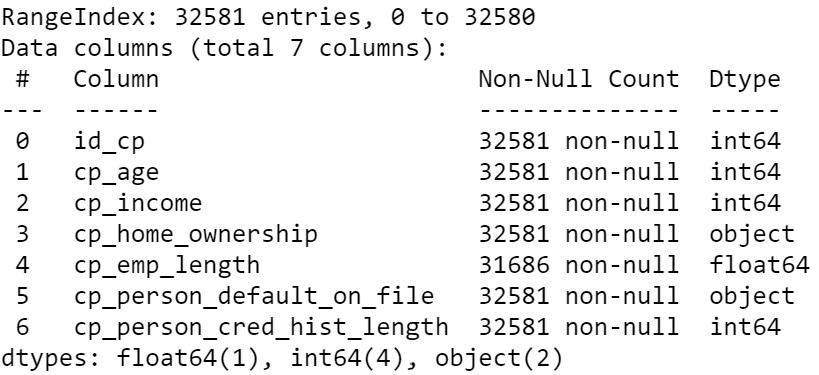
\includegraphics[width=\linewidth]{./images/cp_dataset_info.jpg}
            }
            \caption{\textit{Description of the counterparties' dataset}}
            \label{fig:cp_info}
         \end{figure}
           
    Figure \ref{fig:cp_info} recaps all the information available for counterparties. 
    The variable "employment length" presents some missing values
    that must be handled before proceeding into modelling.
    
        % cp_head FIGURE
        \begin{figure}[H]
            \centerline{
                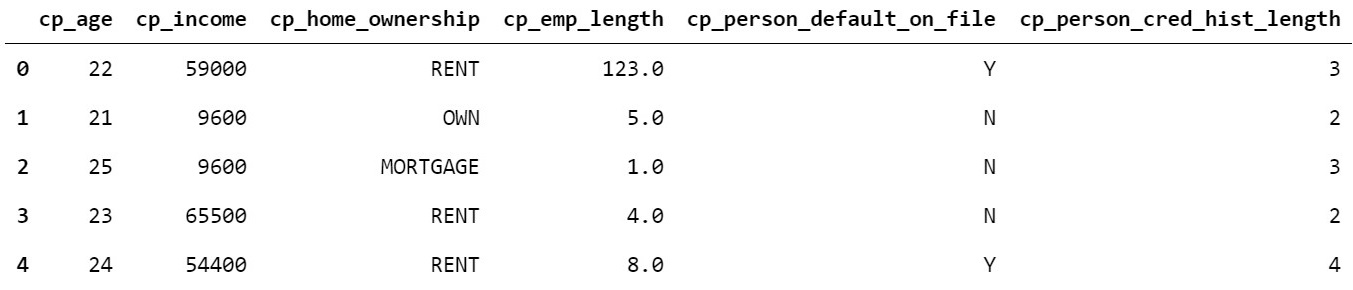
\includegraphics[width=\linewidth]{./images/cp_dataset_head.jpg}
            }
            \caption{\textit{First 5 observations of the counterparties' dataset}}
            \label{fig:cp_head}
        \end{figure}

    The first few observations of the dataset show some inconsistencies with the data: the first observation 
    is characterized by a value for \textit{emplyment length} of 123 years. Let us go into more details:

        % cp_describe FIGURE
        \begin{figure}[H]
            \centerline{
                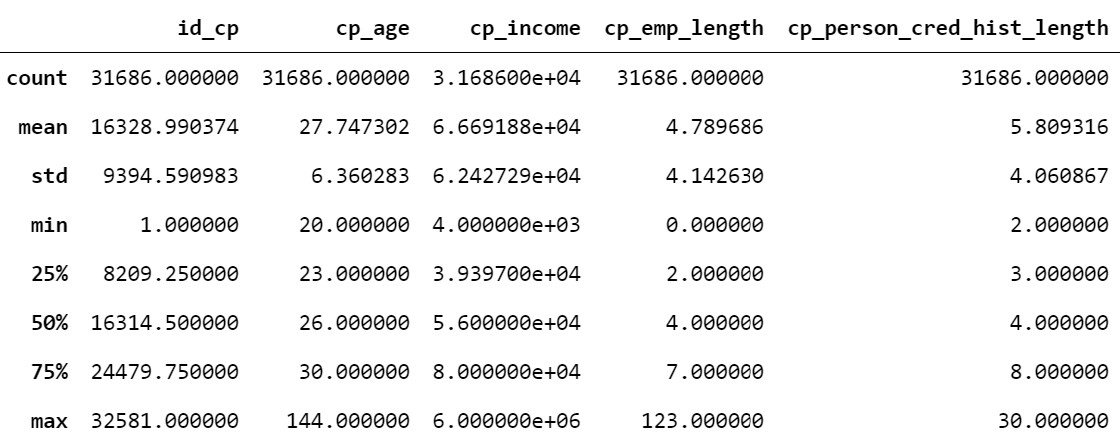
\includegraphics[width=\linewidth]{./images/cp_dataset_describe.jpg}
            }
            \caption{\textit{Statistics on the counterparties' numerical features}}
            \label{fig:cp_describe}
        \end{figure}

    A statistical summary of the numerical features allows us to further inspect the issue with the data, as well
    as having a preliminary assessment of the distribution of each feature. In particular, some inconsistencies 
    in the \textit{age} and \textit{employment lenght} features are spotted and consequently eliminated. 
    A graphical representation of the univariate distribution for each counterparty's features is provided here:

        %cp_univariate FIGURE
        \begin{figure}[H]
            \centerline{
                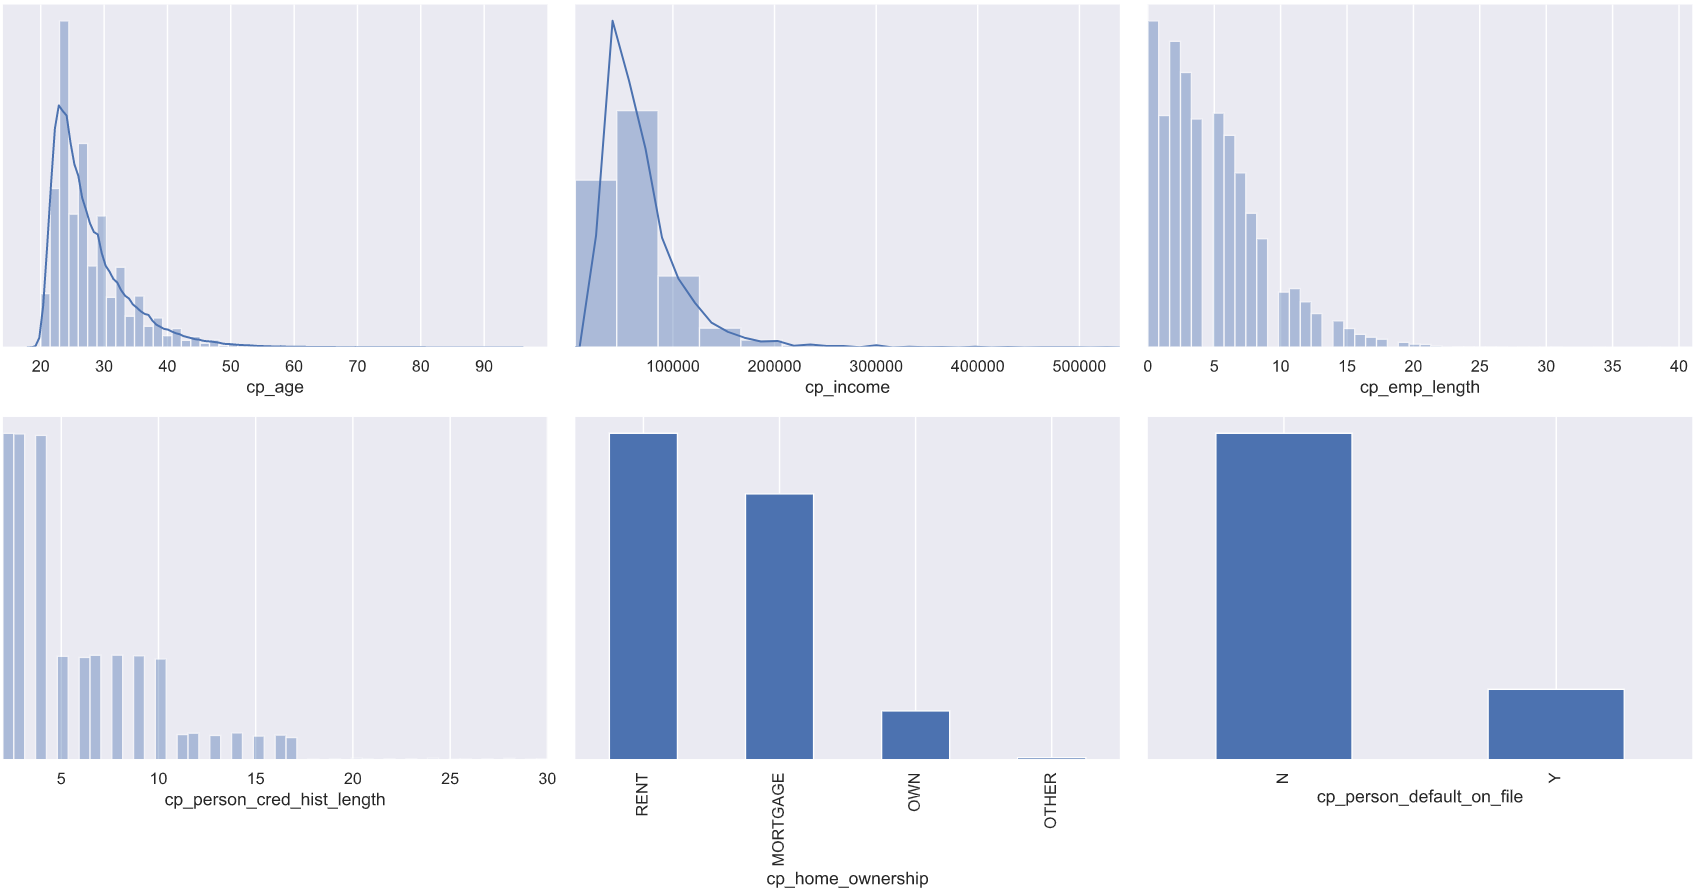
\includegraphics[width=\linewidth]{./images/cp_univariate.png}
            }
            \caption{\textit{Univariate distributions of counterparties' features}}
            \label{fig:cp_univariate}
        \end{figure}

    The following is a list of some of the relevant findings of figure \ref{fig:cp_univariate}:

        \begin{enumerate} 
            \item The set of counterparties is mostly represented by people between their 20s and their 40s. The age distribution seems to have an impact on all the remaining variables. 
            \item Lower age should be the reason for having shorter employment periods and credit history length. In particular, there seems to be a great portion of unemployed people as well as a very large amount of counterparties with little-to-none credit history. Intuitively, unemployment should have a high impact on the assessment of the probability of defaults of a counterparty.  
            \item A very small number of counterparties owns a house, while the majority is either renting or on a mortgage, or in other words, they are already sustaining some debt. Hence, the question here becomes whether these individuals have enough liquidity inflows to sustain another obligation for an extended period. 
            \item The most representative class of counterparties have not defaulted on an obligation in the past. 
        \end{enumerate}

    \subsubsection*{Loans}
    The loans are described by the following 6 features:

    \begin{itemize}
        \item \textit{Loan intent}: the reason to ask for a loan
        \item \textit{Loan grade}: the rating associated with the loan and the relative counterparty. This variable should give us insights on the risk associated with the loan, which is usually driven by the underlying characteristics of the financial instrument (i.e. the loan) as well as the counterparty's characteristics.
        \item \textit{Loan amount}: the amount of the loan
        \item \textit{Loan interest rate}: the interest rate associated with the loan.
        \item \textit{Loan status}: whether the counterparty has defaulted or not on such loan (1 is defaulted, 0 is not) 
        \item \textit{Loan over income}:  the proportion of the loan amount concerning the income of the relative counterparty 
    \end{itemize}

        % loan_info FIGURE
        \begin{figure}[H]
            \centerline{
                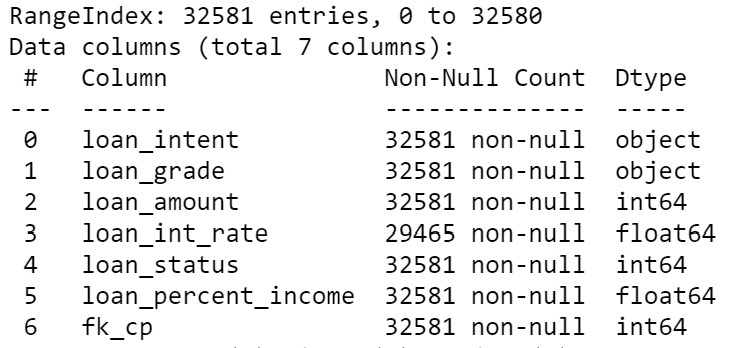
\includegraphics[width=\linewidth]{./images/loans_dataset_info.jpg}
            }
            \caption{\textit{Description of the loans' dataset}}
            \label{fig:loans_info}
         \end{figure}

     The figure \ref{fig:loans_info} gives an overview of the features concering the loans. In particular,
     there is some evidence of the presence of missing values for the \textit{interest rate} variable.
     Moreover, there is a variable called "\textit{fk cp}" which was introduced to reconcile counterparties with loans information.
 
        % loan_head FIGURE
        \begin{figure}[H]
            \centerline{
                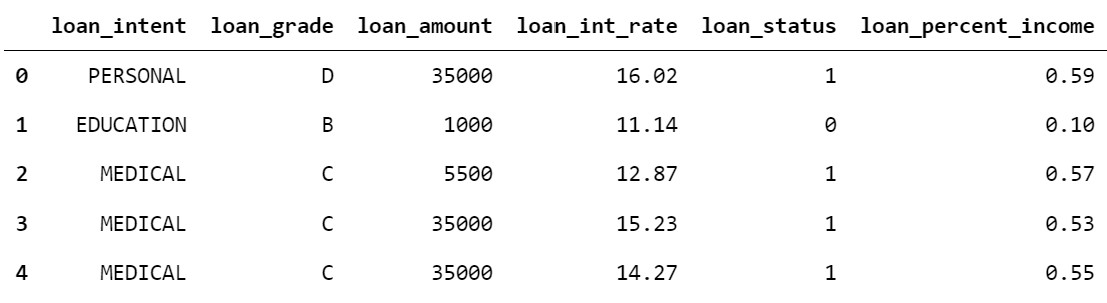
\includegraphics[width=\linewidth]{./images/loans_dataset_head.jpg}
            }
            \caption{\textit{First 5 observations of the loans' dataset}}
            \label{fig:loans_head}
        \end{figure}

     The first few observations of the features describing the loans do not present any relevant concern regarding 
     data inconsistencies. Let's verify if this can be generalized to the entire dataset
     
        % loan_describe FIGURE
        \begin{figure}[H]
            \centerline{
                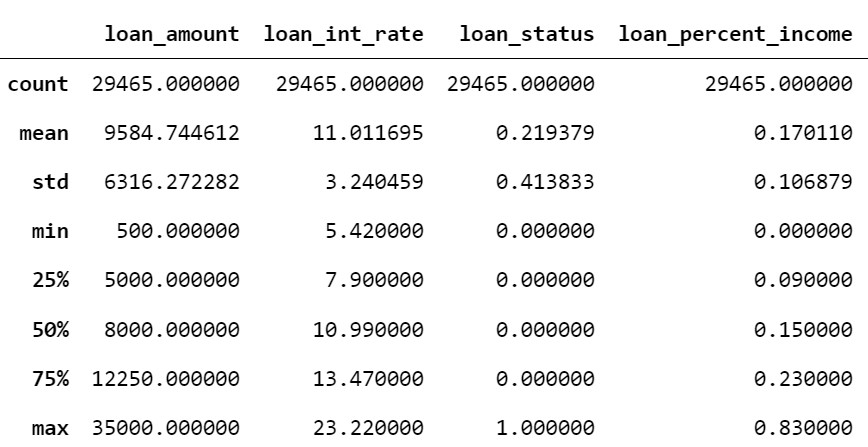
\includegraphics[width=\linewidth]{./images/loans_dataset_describe.jpg}
            }
            \caption{\textit{Statistics on the loans' numerical features}}
            \label{fig:loans_describe}
        \end{figure}

    All the numerical features seem to be within the expected range, with the expection of \textit{loan over income}:
    this variable is calculated dividing the \textit{loan amount} with the \textit{counterparty income}. Hence, having 
    those variables a minimum value greater than 0 simply translates into presence of inconsistencies which can be simply 
    corrected by replacing the entire column with the original calculation.
    
        % loans_univariate FIGURE
        \begin{figure}[H]
            \centerline{
                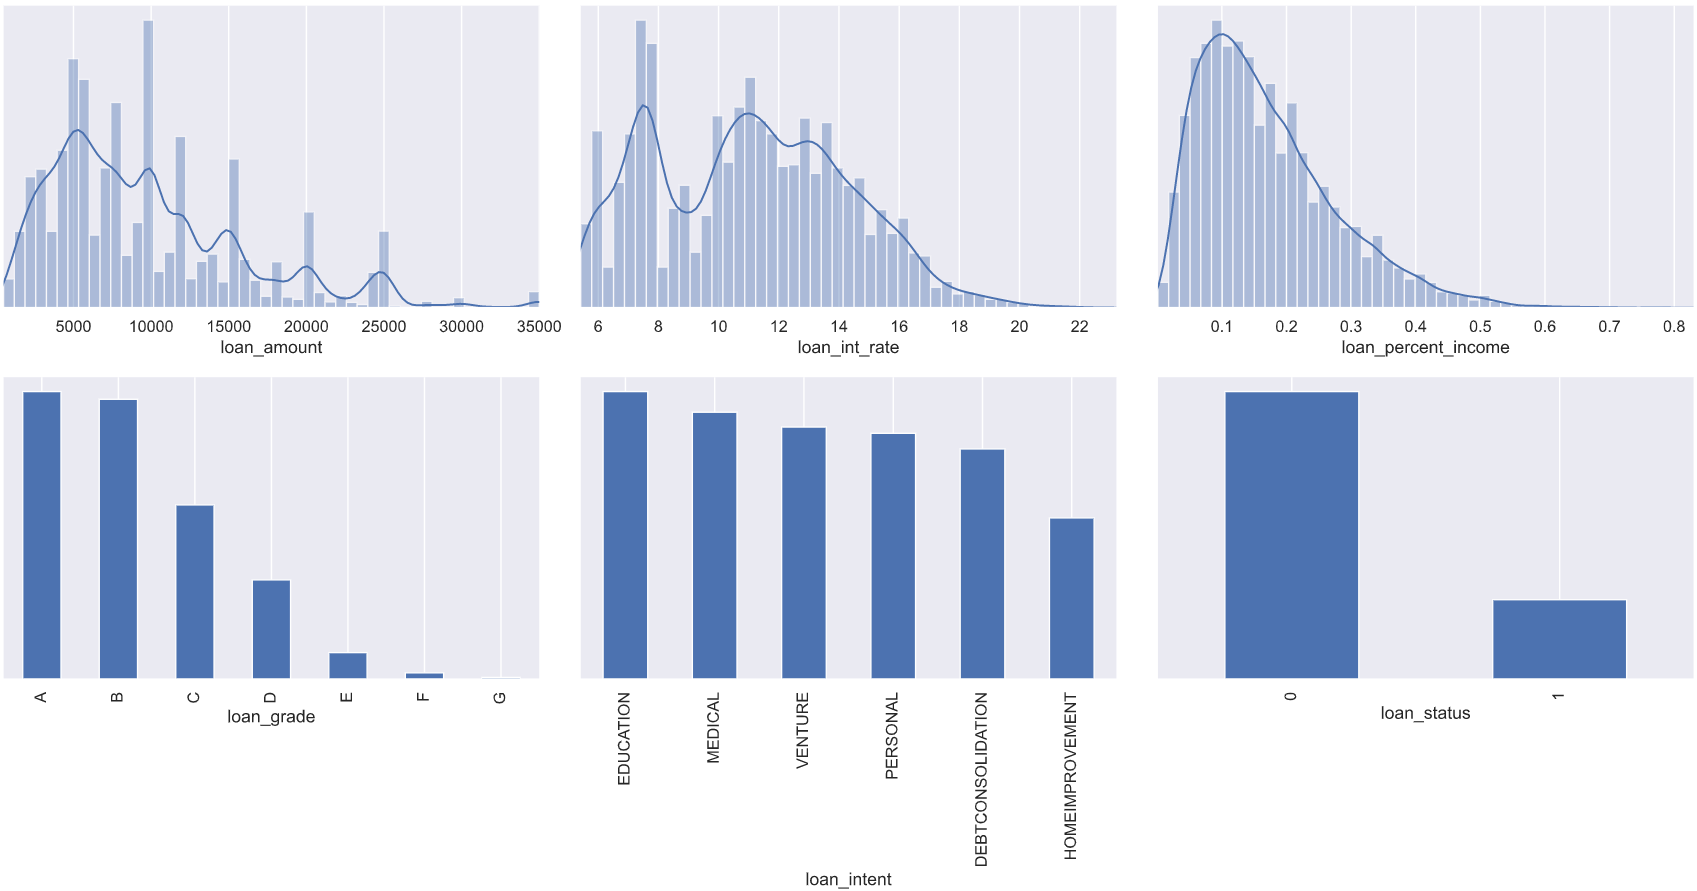
\includegraphics[width=\linewidth]{./images/loans_univariate.png}
            }
            \caption{\textit{Univariate distributions of loans' features}}
            \label{fig:loans_univariate}
        \end{figure}

    The following is a list of some of the relevant findings of the figure \ref{fig:loans_univariate}:
 
        \begin{enumerate} 
            \item The loan amount is mostly concentrated around 5-10K, which is a relatively low number if compared against the distribution of the counterparty's income. 
            \item A great proportion is classified as a "relative safe loan" (i.e. loan grade being either equal to "A", "B" or "C"). Considering this finding, along with the relatively high frequency of non-defaulting loans, it might be the case that the provided PD calibration has already a high degree of accuracy (i.e. the lender can properly distinguish between good and bad obligators).  
            \item Despite a balanced representation of intents, "education" seems to prevail among the reasons to ask for a loan. Debt consolidation usually signals larger debt, lower interest rates, but also a great payment history with the lender. [Julia, 2020]
        \end{enumerate}
 
    \subsubsection{Loan affordability}
    Previous to granting a loan, a lender would like to know whether a counterparty will be able to sustain that loan in the 
    future. To be able to properly assess this, a lender would require details of a counterparty's inflows and outflows 
    as well as short-term future plans. This is usually referred to as "mortgage affordability" [Salih, 2017], as it is frequently used as one 
    of the main determinants of a financial istitutions propensity to extend a mortage. Despite dealing with a more general type of debt
    and not having all the information required, it is possible to define a simplified version of the \textbf{affordability} with the features 
    provided:

        \begin{equation} affordability_{i}=\frac{(loanAmount_{i} * loanIntRate_{i})}{income_{i}}
        \end{equation}

    The following graph provides evidence of the importance of this variable in assessing the probability of default of a counterparty. 
    In particular, it is possible to notice that defaulting loans presents higher affordability values, which translates into greater outflows
    with respect to the income of a counterparty, and intuitevely, higher chances of counterpaties defaulting on such loans.
    
        %affordability FIGURE
        \begin{figure}[H]
            \centerline{
                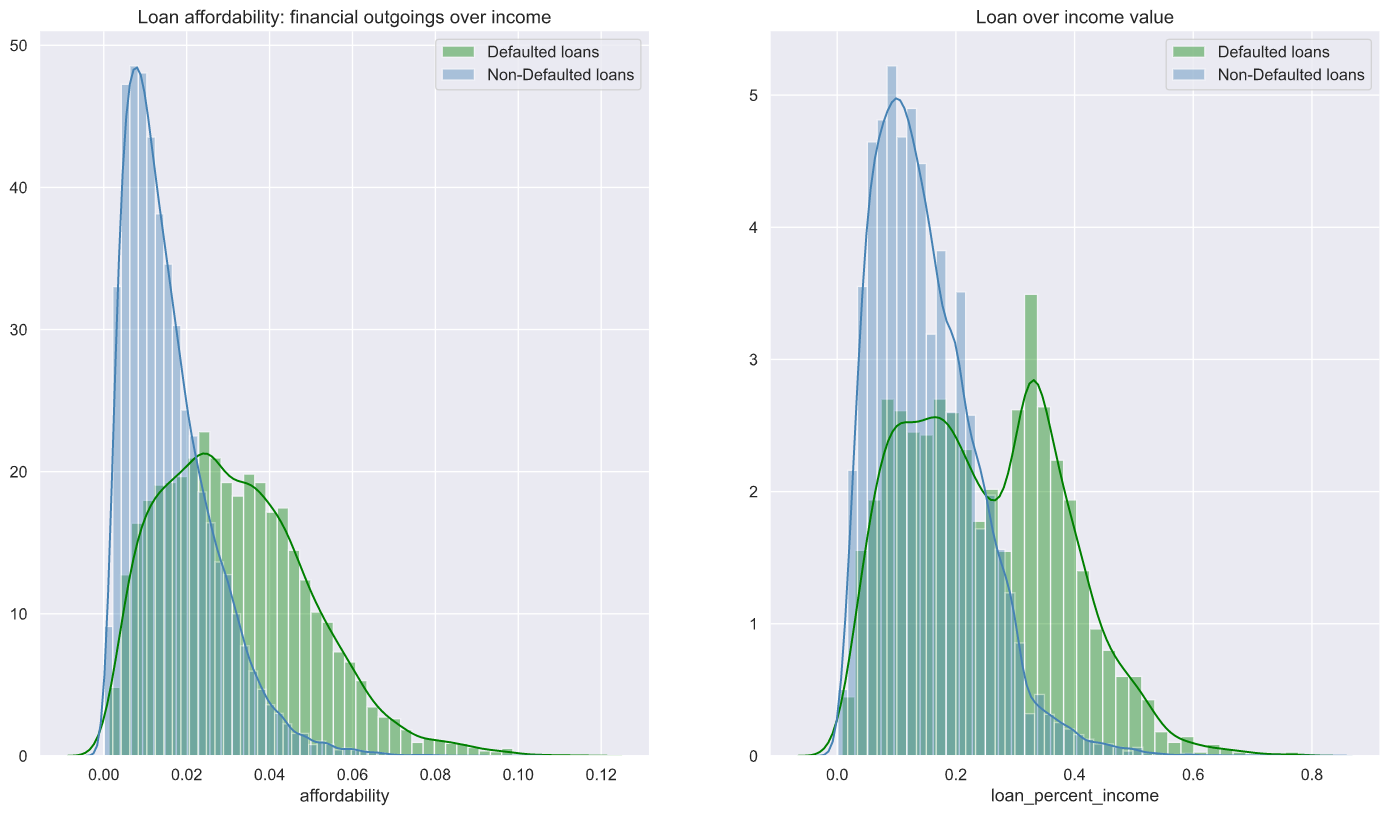
\includegraphics[width=\linewidth]{./images/affordability.png}
            }
            \caption{\textit{Affordability vs. loan-percent-income per loan status}}
            \label{fig:affordability}
        \end{figure}

    Affordability can be seen as a "\textit{normalized version}" of the "loan-percent-income" 
    feature and for sure, much of its variance can be explained by the former variable. 
    Hence, from this point onwards, affordability will be considered in place of "loan-percent-income", 
    but it will not be rejected from the combined analysis.

    %%%%%%%%%%%%%%%%%%%%%%%%%%%%%%%%%%%%%%%%%%%%%%%%%%%%
    % Section (3): Combined analysis
    %%%%%%%%%%%%%%%%%%%%%%%%%%%%%%%%%%%%%%%%%%%%%%%%%%%%    
    \subsection{A combined analysis: between bivariate and multivariate analysis}

    After a standalone overview of the features of counterparties and loans,
    performing a combine analysis is what allow us to inspect how 
    these variables are related to each other.

    \subsubsection{The correlation matrix}
    The correlation matrix is a great starting point for the analysis 
    of the relationships among features. In particular, 
    the \textbf{correlation coefficient} gives an indication of the 
    strength of the \textbf{linear relationship} between 
    two variables [Benesty 2009]. 
    This ranges between $[-1,1]$ based on the intensity of such 
    relationship: if positive (i.e. between $(0,1]$) then the two 
    variables are said to be "positively correlated" or, in other words,
    when one variable increases the other follows and vice versa. 
    If instead, this coefficient is negative (i.e. between $[-1,0)$), 
    then we are in a situation of "inversely related" variables: the 
    increment of one of the two variables causes the other to drop.

    The correlation matrix allows us to extend this analysis for each 
    of the possible combinations of numerical features in our dataset. 

        % correlation_matrix FIGURE
        \begin{figure}[H]
            \centerline{
                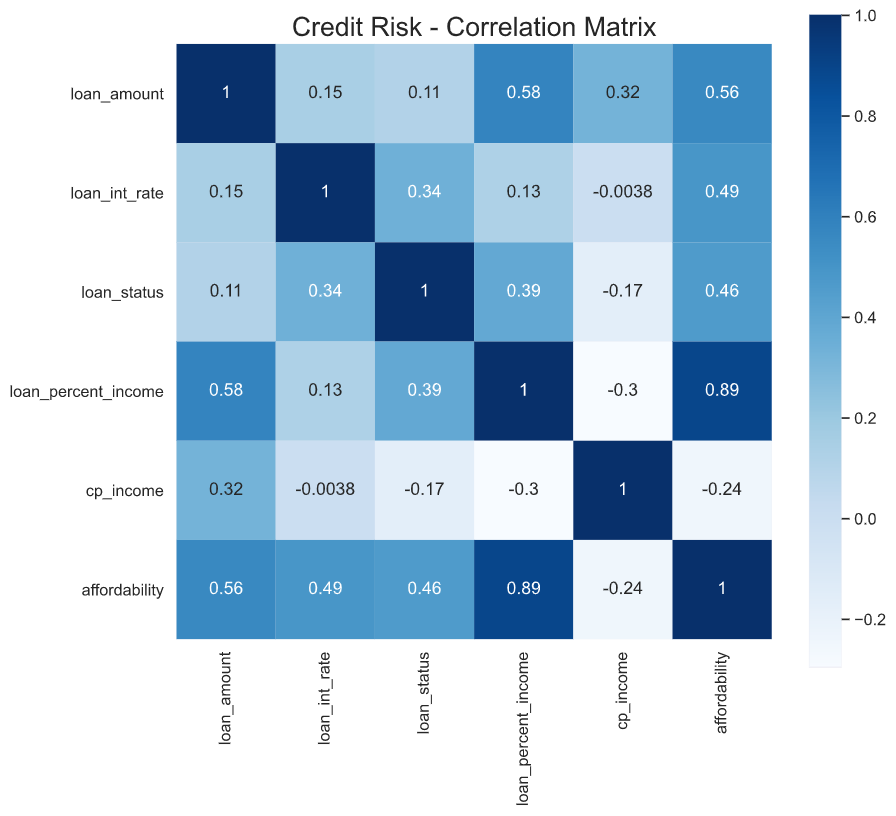
\includegraphics[width=\linewidth]{./images/correlation_matrix.png}
            }
            \caption{\textit{Correlation matrix between loans and counterparties numerical features}}
            \label{fig:corr_matr}
        \end{figure}

    The correlation matrix presented in figure \ref{fig:corr_matr} provides already 
    some key insights that can be summarized in the following points:

    \begin{itemize}
        \item 
        The age of the counterparty drives the relative credit history length. 
        This is quite intuitive, as you would expect that the older a person gets, 
        the more likely it is that this person has been in a credit contract for a longer period.
        \item 
        The ratio "loans over income" is correlated with both "loan amount" and "affordability", 
        which is ultimately correlated with the interest rate.
         When building up a model, we need to make sure that highly 
         correlated variables get excluded from being predictors due to
         multicollinearity issues \texttt{[Alin, 2010]}
        \item The 
        loan amount is indeed correlated with the income of the counterparty
        to which the loan has been given. The intuition behind might 
        be that the higher the income, the more likely it is for this person 
        to sustain even higher repayments in the future 
        (i.e. the principal and the interest rates of the loan)
        \item 
        Lastly, although it is not usually appropriate to include a binary variable in the 
        correlation analysis as it might drive too simplistic conclusions, 
        some surprising results pop up here: the loan status is positively 
        correlated with both interest rate and affordability. 
        The underlying reasoning might be the following:
         since loan status takes value 1 when the counterparty defaults on that loan, 
         the higher the financial outgoings concerning the counterparty's income, 
         the more likely it gets that a counterparty default on this loan.
    \end{itemize}

    Linear relationships are a great starting point to explore how variables are related among each other. 
    Proceeding, we might want to see whether there are some other trends that we can capture exploting other tools. 
    

    % CREDIT HISTORY
    \subsubsection{What does a counterparty's defaulting history can tell?}
    The feature "\textit{cp-person-default-on-file}" gives information on the credit history of a counterparty which, in turn, 
    should also provide some evidence on the creditworthiness of a client. 
   
        % figure CROSSTAB DEFAULTS GRADE
        \begin{figure}[H]
            \centerline{
                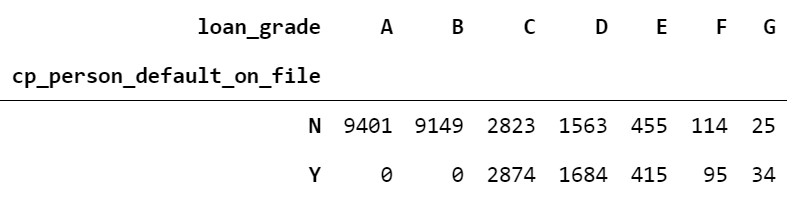
\includegraphics[width=\linewidth]{./images/loans_ct_grades_credit_history.jpg}
            }
            \caption{\textit{Number defaulted (Y) and non-defaulted (N) counterparties per loan grade}}
            \label{fig:tab_defaults_grade}
        \end{figure}

    The result from figure \ref{fig:tab_defaults_grade} is not surprising and highlights also a trend: 
    the expectations are that a lender should issue more high-graded loans to people that did not already default in the past 
    (i.e. with a better credit history ("\textit{cp-person-default-on-file = N}") and less low-grade and riskier loans to people with a worse credit history. 
    Another approach could consist in exploring how this flag relate to the dependent variable: \textbf{loan status}.

        % figure LOAN STATUS vs DEFAULTING HISTORY
        \begin{figure}[H]
            \centerline{
                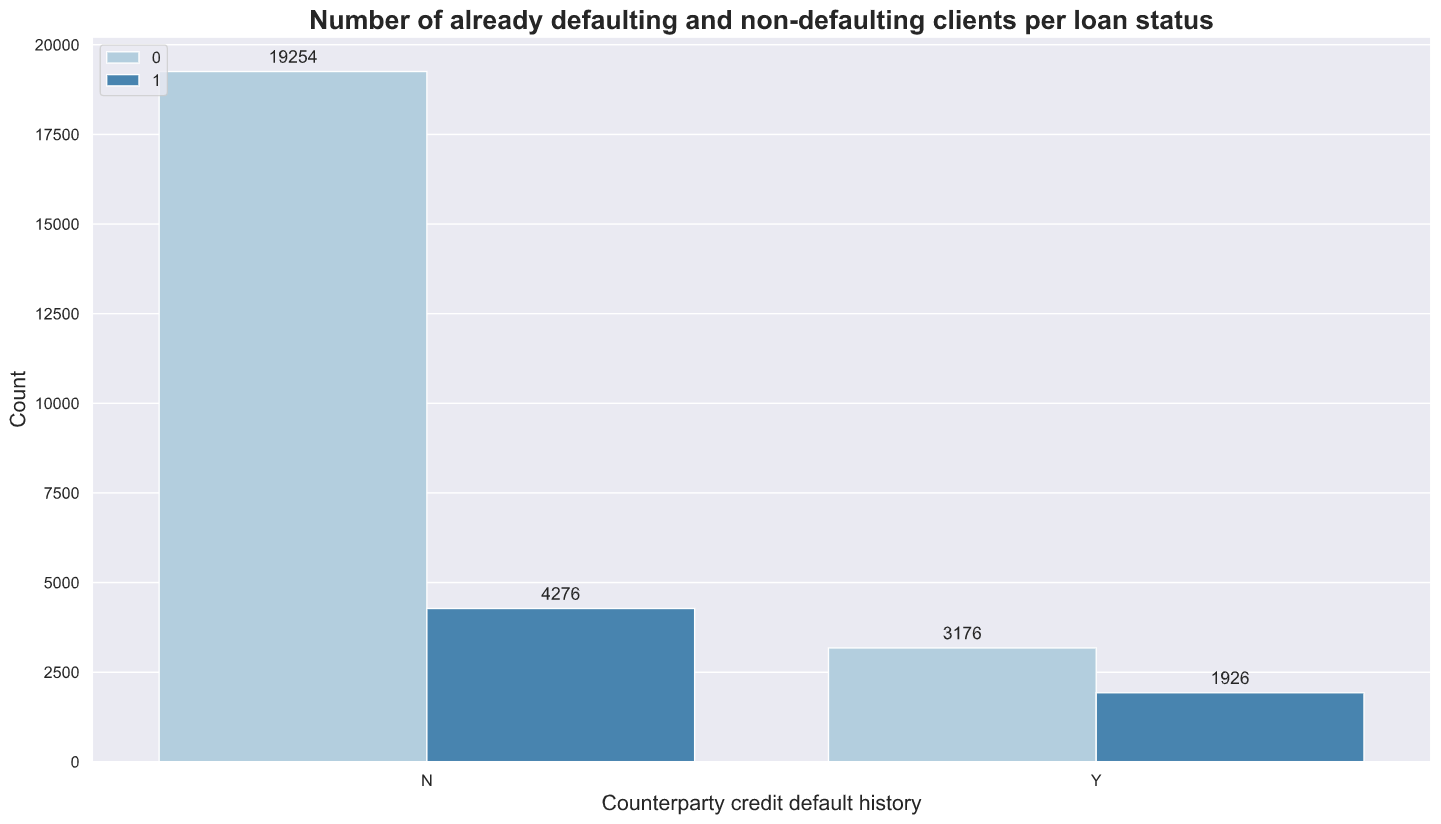
\includegraphics[width=\linewidth]{./images/loans_status_credit_history.png}
            }
            \caption{\textit{Number defaulted (Y) and non-defaulted (N) counterparties per loan status}}
            \label{fig:hist_status_credit_history}
        \end{figure}
    
    Figure \ref{fig:hist_status_credit_history} shows that a significant proportion of non-defaulting loans is held by counterparties with good credit history. 
    Nevertheless, most of the defaulting loans belong to counterparties that did not default in the past. 
    This might be due to several factors that go out of the scope of this empirical analysis (e.g. softened controls, 
    counterparties underlying characteristics, presence of asymmetric information between the two parties). 
    What should be kept in mind is that, although representing counterintuitive results, this variable should turn to be relevant for modelling. 

    To sum up, it seems that a great number of obligators defaulted for the first time (18\%) , 
    but there is a larger proportion (38\%) of counterparties that defaulted for the second time. 
    Let's explore these findings more closely:
  
        % figure MEAN DIFF INT RATE
        \begin{figure}[H]
            \centerline{
                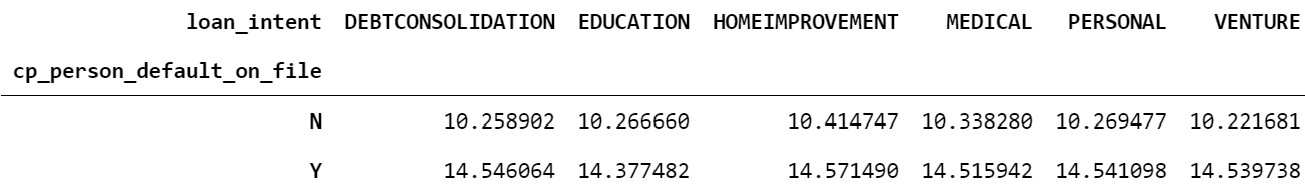
\includegraphics[width=\linewidth]{./images/loans_intents_credit_history_int_rate.jpg}
            }
            \caption{\textit{Interest rates per defaulted (Y) and non-defaulted (N) counterparties across intents}}
            \label{fig:loans_intents_credit_history_int_rate}
        \end{figure}
    
    The \textbf{average} premium difference between counterparties with good and bad credit history is of 422 BP (i.e. 4.22\%). 
    This difference should be also reflected in the distribution of the client's affordability per status across the 
    various reasons to ask for a loan

        % figure AFFORDABILITY - STATUS - INTENTS
        \begin{figure}[H]
            \centerline{
                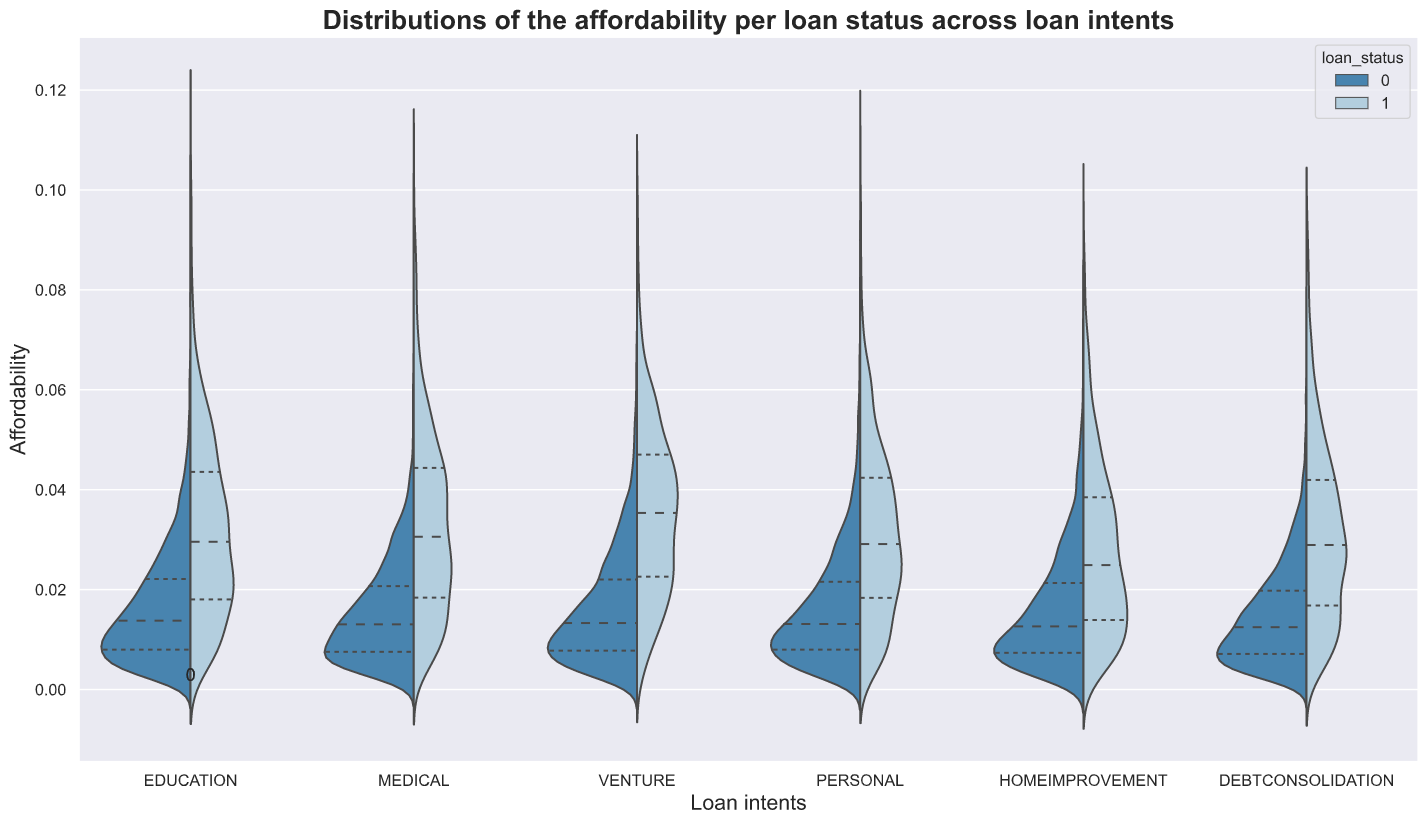
\includegraphics[width=\linewidth]{./images/loans_affordability_status_intents.png}
            }
            \caption{\textit{Affordability distribution per loan status across loan intents}}
            \label{fig:loans_affordability_status_intents}
        \end{figure}

    From the figure \ref{fig:loans_affordability_status_intents} it is indeed possible to find evidence of the hypothesis: 
    the distribution of \textit{affordability} for defaulting clients is shared between categories 
    but differs quite significantly to that for non-defaulting clients. The latter is more concentrated towards much lower numbers. 


    % CALIBRATION
    \subsubsection{PD Calibration: average interest rate for each rating?}
    We wish to explore the relationship between the interest rate and the loan grade, 
    something that was previously introduced with the name of \textbf{calibration} [Bluhm, 2016]. 
    The expectations are that letters towards A should have lower rates, while those further away in the alphabet 
    should represent loans with a much higher rate on average

        % figure AVG.INT RATE - GRADES
        \begin{figure}[H]
            \centerline{
                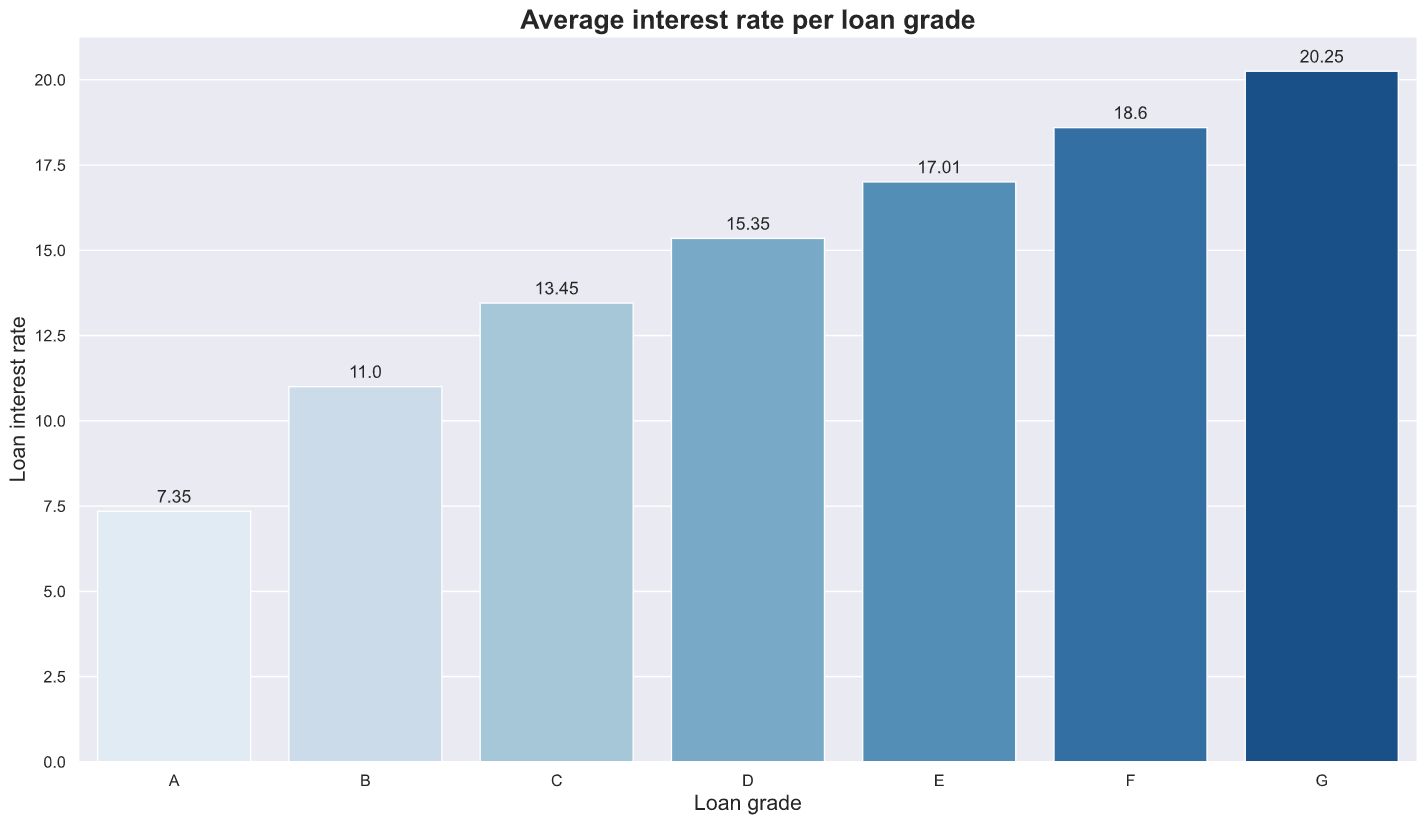
\includegraphics[width=\linewidth]{./images/loans_pd_calibration_hist.png}
            }
            \caption{\textit{Histogram of the average interest rate per loan grade}}
            \label{fig:loans_pd_calibration_hist}
        \end{figure}
    
    The trend highlighted in figure \ref{fig:loans_pd_calibration_hist} is reflected also in the data: the average premium charged to counterparties 
    increases the riskier the loans become. The following graph aims at exploring whether this difference is 
    also reflected for the counterparty's affordability across the two categories of counterparties' credit history (i.e. good or bad obligators).

        % figure AFFORDABILITY - STATUS - CP HISTORY
        \begin{figure}[H]
            \centerline{
                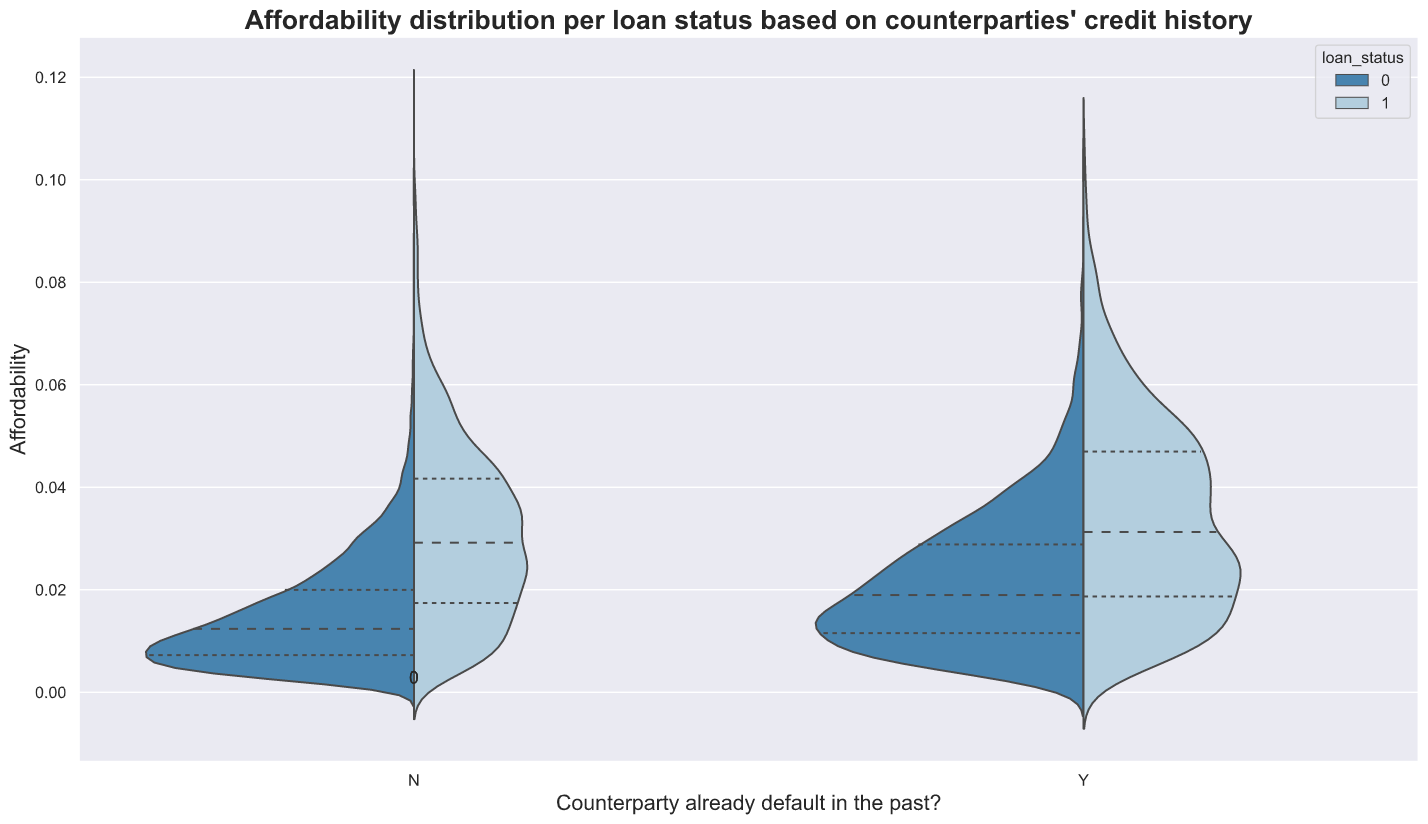
\includegraphics[width=\linewidth]{./images/loans_affordability_status_credit_history.png}
            }
            \caption{\textit{Affordability distribution per loan status based on the credit history of counterparties}}
            \label{fig:loans_affordability_status_credit_history}
        \end{figure}

    Figure \ref{fig:loans_affordability_status_credit_history} seems to confirm the statement presented above: 
    counterparties who already defaulted in the past (i.e. bad obligators) seem to have higher 
    repayments to sustain, independently of the loan status.

    % MORTGAGES AND RENTS
    \subsubsection{A closer look at mortgaged and renting counterparties}
    We want to turn now the attention towards counterparties' ownership status, with particular consideration 
    for those that are on a mortgage or rent which represent more than 90\% of the overall number of entries.
    Indeed, limited to the information we have on counterparties, possessing a house should be enough to 
    demonstrate that the contractual agreements will be met. On the other hand, mortgages and rents represent debt repayments 
    (i.e. future financial outgoings) that the obligator must sustain and therefore the likelihood of defaulting 
    on the loan should raise consequently.

        % figure AFFORDABILITY - STATUS - HOME OWNERSHIP
        \begin{figure}[H]
            \centerline{
                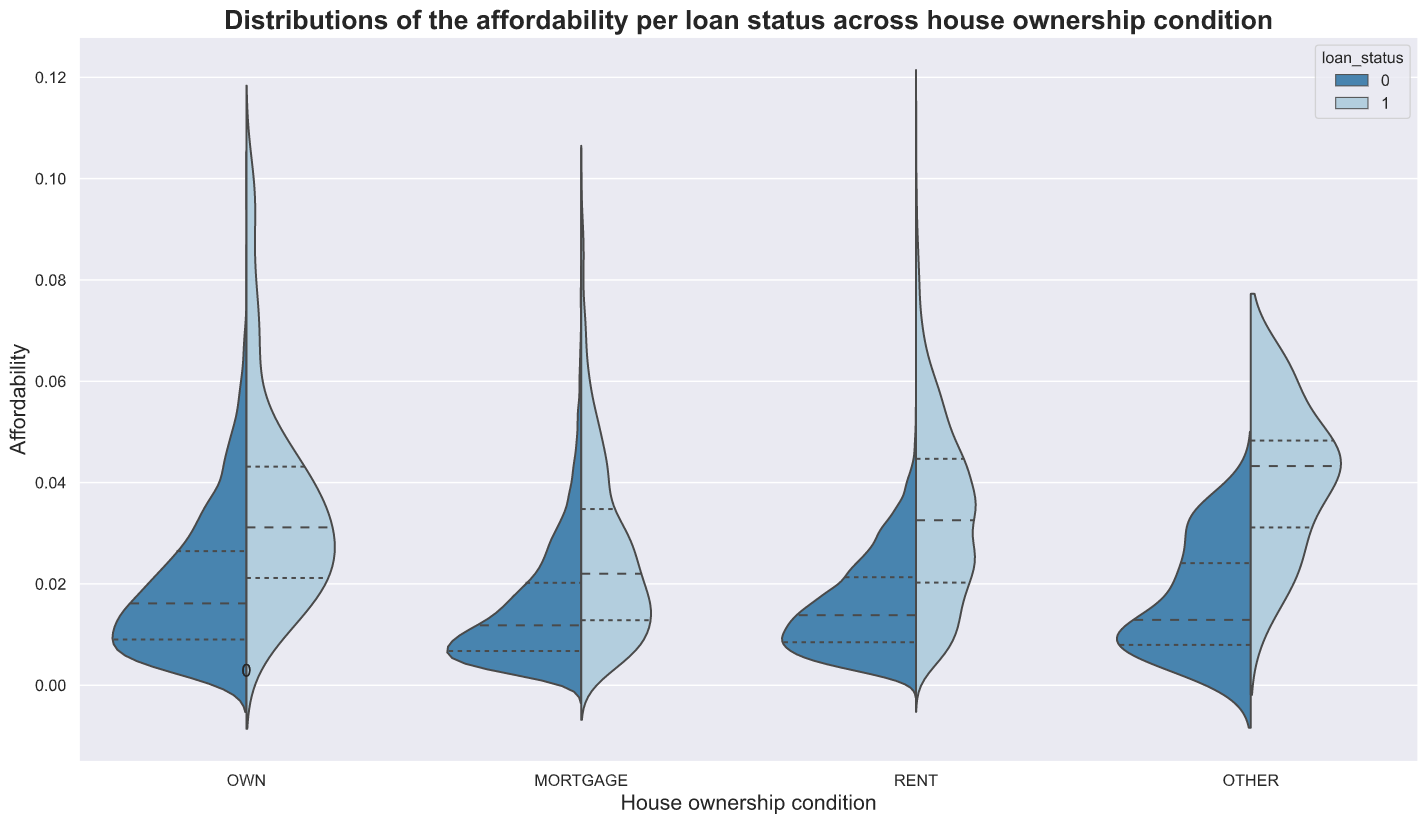
\includegraphics[width=\linewidth]{./images/loans_affordability_status_ownership.png}
            }
            \caption{\textit{Affordability distribution per loan status based on house ownership condition}}
            \label{fig:loans_affordability_status_ownership}
        \end{figure}

    The hypothesis presented above seems not to be confirmed by the empirical results shown in figure \ref{fig:loans_affordability_status_ownership}. 
    Indeed,  the distribution of the affordability for defaulting clients does not seem to vary much across categories of 
    ownership, except for the option "\textit{other}". Note however that the information on the number of 
    financial outgoings of each counterparty is missing from the dataset, and therefore, assessing this 
    statement becomes a much harder job.

    % AGE
    \subsubsection{Do age differences impact the probability of default}
    We already discussed how the age of a counterparty seems to affect the underlying distribution of 
    many other variables in the dataset (to name a few: income, loan intents, credit history). 
    Does it also have an impact on the dependent variable?

    % figure AFFORDABILITY - STATUS - AGE
        \begin{figure}[H]
            \centerline{
                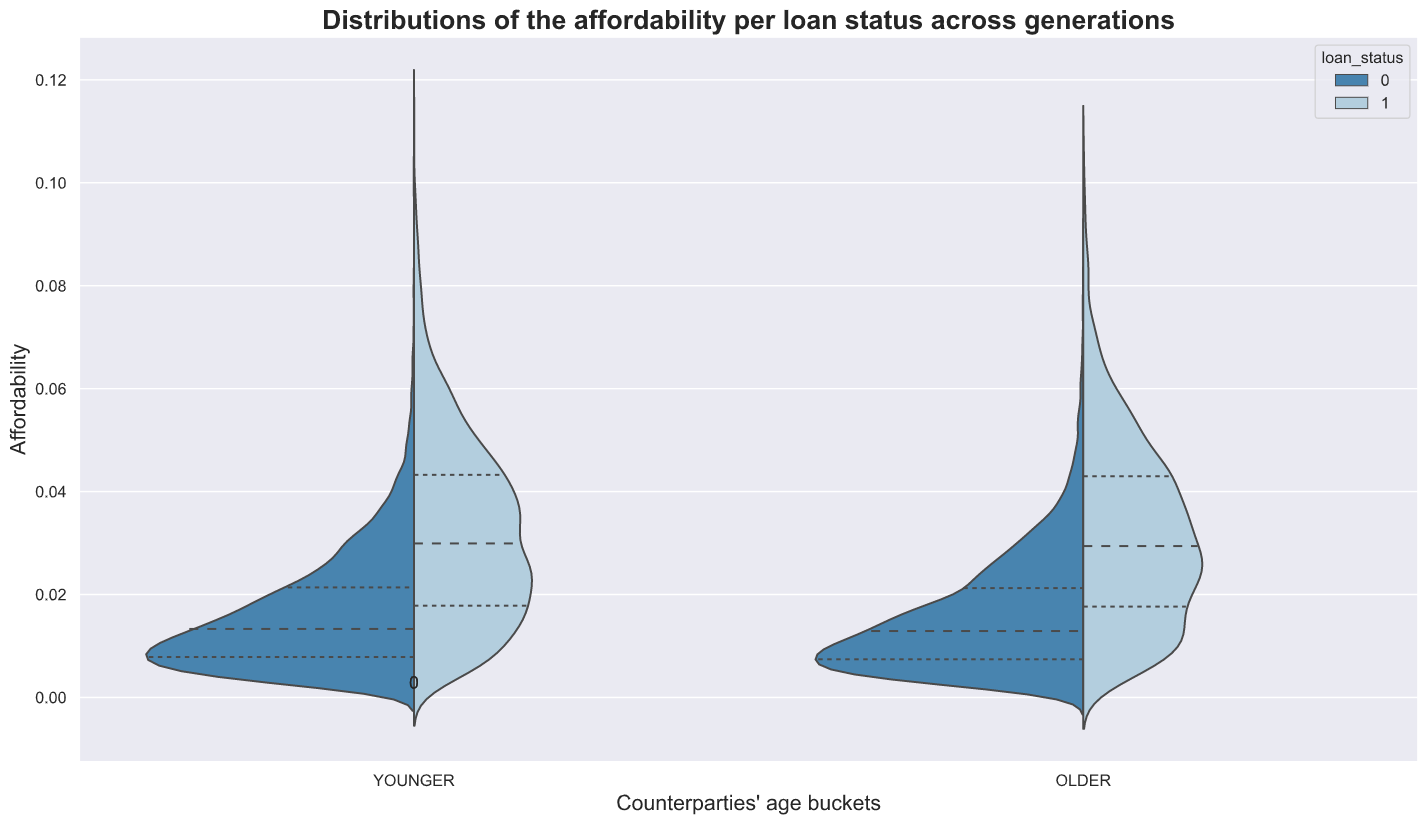
\includegraphics[width=\linewidth]{./images/loans_affordability_status_age.png}
            }
            \caption{\textit{Affordability distribution per loan status based on counterparty's age}}
            \label{fig:loans_affordability_status_age}
        \end{figure}

    Figure \ref{fig:loans_affordability_status_age} reports that affordability is different 
    between defaulting and non-defaulting loans, but does not vary across age buckets. 
    Hence, it seems that our hypothesis ought to be rejected.

    %%%%%%%%%%%%%%%%%%%%%%%%%%%%
    % DATA PREPARATION!
    %%%%%%%%%%%%%%%%%%%%%%%%%%%%
    \subsection[]{Data Preparation}
    \label{sec:data_preparation}

    This section introduces one of the most critical and important processes when it comes to 
    developing an end-to-end machine-learning solution: \textbf{Feature engineering and Selection}. 
    This activity usually comes right before proceeding into modelling to feed the model with a 
    dataset that best suits the purpose.  Quoting [Hannah, 2019]: 
    "\textit{in machine learning the model is only ever as good as the data it is trained on. 
    As such, a significant proportion of the effort should be focused on creating 
    a dataset that is optimised to maximise the information density of the data"}. 
    In other words, making sure that the data respects all the model assumptions and 
    that is presented in the most suitable form before the model gets trained is crucial. 
    The approach taken in this analysis is as follow:

        \begin{enumerate}
            \item \textbf{Feature engineering: Variable discretization }
            \item \textbf{Features dropping: loan-percent-income and loan-grade}:
            \item \textbf{Handling categorical features: dummy transformation}
            \item \textbf{Dealing with unbalancedness: SMOTE algorithm}
            \item \textbf{Features selection: RFE approach}
            \item \textbf{Protect against multicollinearity issues: VIF measure}
        \end{enumerate}

        % FEATURES ENGINEERING
        \subsubsection{Feature engineering}
        The features \textit{age}, \textit{employment length} and \textit{credit history} 
        have been discretized based on a method called \textbf{equal-frequency discretization} [Charfaoui, 2020]. 
        In particular, the range of possible values of each of these features is divided into 
        "\textit{N bins}", each holding approximately the same number of observations. 
        Indeed, the split is made according to the underlying distribution of the feature, 
        where the interval boundaries correspond to the quantiles. Such a procedure should 
        bring multiple benefits for the modelling part. Among these, the most important are [Charfaoui, 2020]:

        \begin{itemize}
            \item Improvements of the value spread of the variable
            \item Outliers handling
            \item When combined with categorical encodings, chances are that this method should improve the predictive power of the model 
        \end{itemize}
        
        % FEATURES DROPPING
        \subsubsection{Feature dropping}
        The reasons why loan-percent-income and loan-grade features have been a drop 
        from the modelling dataset should be taken separately:

            \begin{itemize}
                \item \textit{loan-percent-income}: figure \ref{fig:corr_matr} reports a correlation coefficient of \textbf{0.89} between this feature and affordability. According to [Molala, 2019], a value greater or equal than 0.7 highlights the presence of multicollinearity which is something we wish to avoid among predictors. The reason for this will be given later under the section "\textit{protect against multicollinearity issues}"
                \item \textit{loan-grade}: the motivation for the drop is related to the way this feature is built up, and more precisely, to the \textbf{calibration} process. We have already seen in chapter \ref{sec:calibration} that calibration is the process of assigning a default probability to a grade based on past information of the default rates for each rating [Bluhm, 2016]. Therefore, using loan grade as a predictor would likely inject prior information on the default probabilities of each loan according to the rating class that was assigned to them. This would surely increase the performance of the model, but would also increase the likelihood of overfitting on the data at hand. Hence, the variable is excluded from being a predictor of the default probability 
            \end{itemize}

        % DUMMIES
        \subsubsection{Handling categorical features}
        The motivation for handling categorical features is that most machine learning
        models cannot work directly with these features and therefore they need to be converted into numerical values. 
        The approach adopted here is called: \textbf{dummy transformation}: a number of columns equal
        to the unique cases of each categorical feature taken separately will be generated, and each of 
        these columns will take value 1 if the observation takes the value represented by that column, otherwise 0.
        Note that to avoid multicollinearity issues one column for each original feature must be excluded from the 
        dataset and used as a base case to interpret the coefficients [Mahto, 2019].

        % SMOTE: Oversampling
        \subsubsection{Dealing with unbalancedness}
        Figure \ref{fig:hist_status_credit_history} shows that the dependent variable \textit{loan-status} in 
        \textbf{unbalanced}: there are much more observations for non-defaulting loans (i.e. \textit{loan-status=0}) than for the other (i.e. \textit{loan-status=1}).
        Is there a problem with such a finding? Responding to a similar question, [Aedula, 2017] highlights the issue in a very simplistic manner:
        "\textit{if you train your classifier without balancing the classifier has a high chance of favouring one of the classes with the most examples}".
        In other words, if we were to train a model leaving the dataset as it is, it might as well be the case that the model is biased towards non-defaulting loans and even when there is enough evidence to classify an observation as defaulting (i.e. \textit{loan-status=1}), the model would go for the opposite. The solution to this problem is called "\textbf{over-sampling}" which, in practical terms, can be implemented using 
        \textbf{SMOTE ((Synthetic Minority Over-sampling)}  [Chawla, Bowyer, Hall, Kegelmeyer, 2002]. 
        Essentially, this algorithm performs two fundamental operations [Li, 2017]:

        \begin{itemize}
            \item Randomly extracts a sample and considers the \textit{K-Nearest Neighbors} [Peterson, 2009]
            \item Use the K-Nearest Neighbors to create similar, but randomly tweaked, new observations for the minority class (i.e. \textit{loan-status=1})
        \end{itemize}

        The result will consists in an "oversampled" dataset having the same number of observations for what 
        was previously identified as the minority class \textit{loan-status = 0}) and the majority class (i.e. \textit{loan-status = 0})

        % RFE: Recursive Feature Selection
        \subsubsection{Features selection}
        After having applied all the transformations deemed necessary to properly train a model for a binary classification problem, another 
        important aspect to consider is to pick the features that are most relevant to model for our dependent variable. 
        To accomplish this task, we will make use of the \textbf{RFE (Recursive Feature Elimination)} algorithm [Scikit-learn RFE, 2020].
        The description of the latter goes as follow: given an estimator (e.g. logistic regression model) the algorithm proceeds in recursively 
        evaluating the performance on smaller and smaller sets of features and, 
        based on the \textit{coefficient} and \textit{feature importance} attributes, the least important ones 
        are pruned until the desiderable number of features is eventually reached.  
        
            % figure RFE            
            \begin{figure}[H]
                \centerline{
                    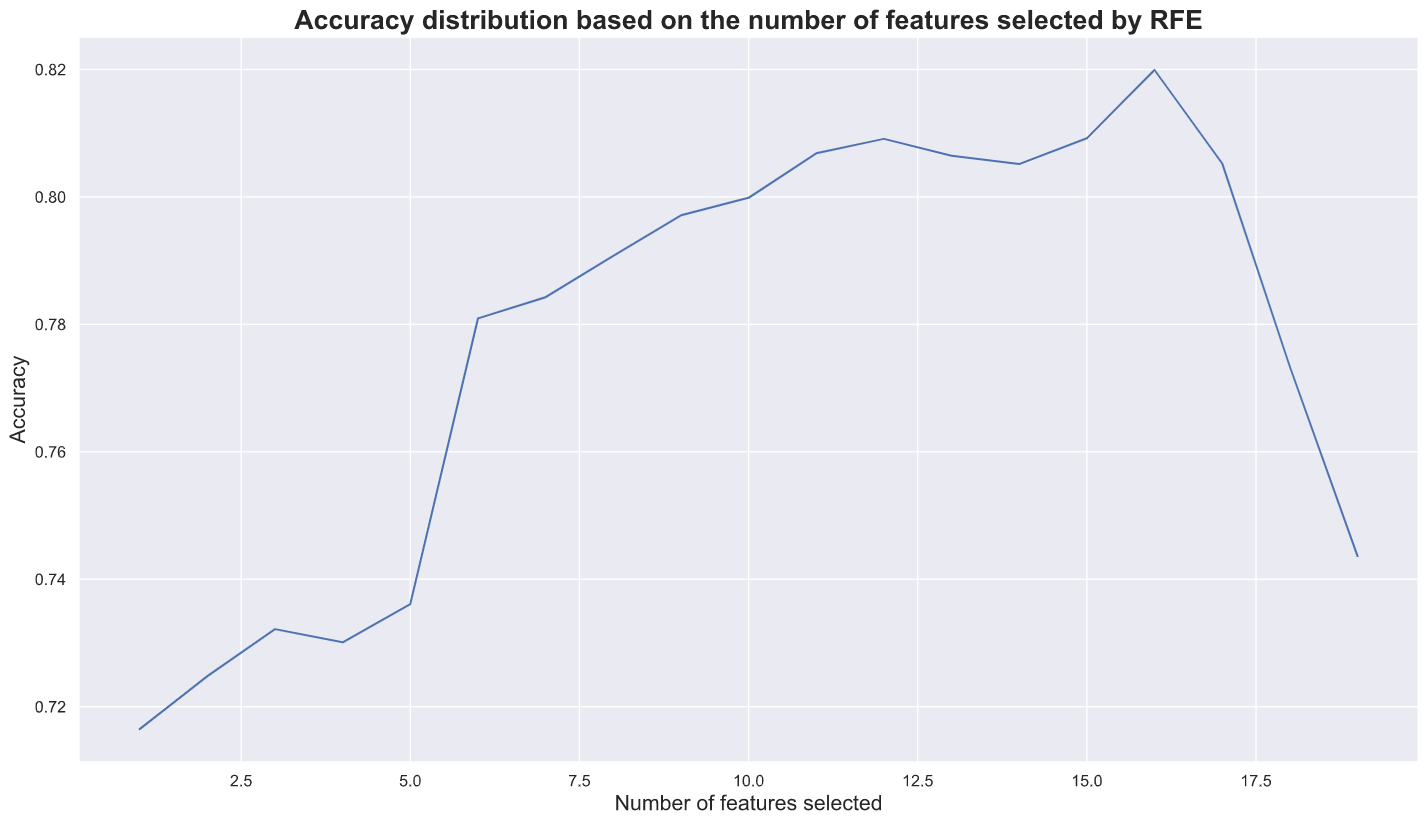
\includegraphics[width=\linewidth]{./images/model_features_RFE.png}
                }
                \caption{\textit{Accuracy distribution based on the number of features selected by RFE}}
                \label{fig:RFE}
            \end{figure}


        Looking at figure \ref{fig:RFE} it is possible to notice that, when picking the most relevant features, what the algorithm does 
        in the background is to try optimize for a pre-defined metric, which in this case was set to be \textbf{accuracy}.
        The set of features picked by the algorithm  might not be the ones eventually used to to train the model,
        as this procedure does not take \textbf{directly} into consideration other relevant aspect for this purpose, such as that of \textbf{multicollinearity}.

        % VIF: Variance Influence Factor as a measure of multicollinearity
        \subsubsection{Protect against multicollinearity issues}
        One of the core assumption in a binary classification problem is that predictors should be independent from each other or,
        in other words, that there is no presence of \textbf{multicollinearity} among features. 
        Multicollinearity refers to a situation in which two or more explanatory variables are highly linearly related. [Fox, John, and Georges Monette] 
        \textbf{VIF (Variance Inflation Factor)} is one of the most frequently used metric to measure such phenomenon, as it 
        provides and index that enables to quantify the severity of multicollinearity among features in the context of linear models.
        The value \textbf{5} is commonly used as a \textit{cutoff value} to indicate the presence of high multicollinearity. 
        A feature having a VIF greater than 10 is recognized to have serious issues of multicollinearity and 
        should be then excluded from the dataset. Note that the value \textbf{5} is also commonly used as a cutoff value for 
        the presence of multicollinearity [VIF Wikipedia, 2010]. 

        The following figures highlight the procedure used to get rid of multicollinearity issues among the features 
        selected by the recursive feature elimination algorithm.

            % figure VIF (entire dataset)
            \begin{table}[H]
                \centering
                    \begin{tabular}{|c | c|} 
                        \hline
                            Feature & VIF \\ [0.5ex] 
                            \hline\hline
                            \texttt{loan-amount} & 8.75 \\
                            \texttt{loan-int-rate} & 10.28 \\
                            \texttt{cp-income} & 4.92 \\
                            \texttt{affordability} & 10.07 \\
                            \texttt{loan-intent-EDUCATION} & 1.42 \\
                            \texttt{loan-intent-HOMEIMPROVEMENT} & 1.28 \\
                            \texttt{loan-intent-MEDICAL} & 1.42 \\
                            \texttt{loan-intent-PERSONAL} & 1.38 \\
                            \texttt{loan-intent-VENTURE} & 1.41 \\
                            \texttt{cp-home-ownership-OTHER} & 1.01 \\
                            \texttt{cp-home-ownership-OWN} & 1.17 \\
                            \texttt{cp-home-ownership-RENT} & 2.39 \\
                            \texttt{cp-person-default-on-file-Y} & 1.31 \\
                            \texttt{cp-emp-title-MIDDLE} & 1.48 \\
                            \texttt{cp-emp-title-SENIOR} & 1.59 \\
                            \texttt{cp-emp-title-UNEMPLOYED} & 1.23 \\
                            \texttt{cp-cred-period-MEDIUM} & 2.06 \\
                            \texttt{cp-cred-period-LONG} & 3.37 \\
                            \texttt{cp-age-bucket-OLDER} & 3.73 \\ [1ex]
                        \hline
                    \end{tabular}
                    \caption{\textit{VIF - whole dataset}}
                    \label{table:VIF_general}
            \end{table}

            Considering all the features of the dataset and a cutoff value for VIF equal to 5, it seems
            that we have serious issues of multicollinearity. Let's see what happens if we consider only
            the features picked by the RFE algorithm:

            % figure VIF (RFE-based dataset)
            \begin{table}[H]
                \centering
                    \begin{tabular}{|c | c|} 
                        \hline
                            Feature & VIF \\ [0.5ex] 
                            \hline\hline
                            \texttt{loan-int-rate} & 7.29 \\
                            \texttt{affordability} & 4.16 \\
                            \texttt{loan-intent-EDUCATION} & 1.40 \\
                            \texttt{loan-intent-HOMEIMPROVEMENT} & 1.27 \\
                            \texttt{loan-intent-MEDICAL} & 1.41 \\
                            \texttt{loan-intent-PERSONAL} & 1.37 \\
                            \texttt{loan-intent-VENTURE} & 1.40 \\
                            \texttt{cp-home-ownership-OTHER} & 1.01 \\
                            \texttt{cp-home-ownership-OWN} & 1.16 \\
                            \texttt{cp-home-ownership-RENT} & 2.33 \\
                            \texttt{cp-person-default-on-file-Y} & 1.30 \\
                            \texttt{cp-emp-title-MIDDLE} & 1.46 \\
                            \texttt{cp-emp-title-SENIOR} & 1.53 \\
                            \texttt{cp-emp-title-UNEMPLOYED} & 1.23 \\
                            \texttt{cp-cred-period-MEDIUM} & 1.60 \\
                            \texttt{cp-cred-period-LONG} & 1.49 \\ [1ex]
                        \hline
                    \end{tabular}
                    \caption{\textit{VIF - features picked by the RFE algorithm}}
                    \label{table:VIF_RFE}
            \end{table}

            The RFE algorithm picked 16 variables and excluded most of those that were causing 
            multicollinearity issues: \textit{loan-amount}, \textit{cp-income} and \textit{age}.
            Nevertheless, \textit{loan-interest-rate} was picked as a relevant feature, but the VIF value
            suggests (using a cutoff of 5) that the variable should be drop from the dataset due to the 
            presence of multicollinearity.

            % figure VIF (Manually exluded features based on previous VIF result)
            \begin{table}[H]
                \centering
                    \begin{tabular}{|c | c|} 
                        \hline
                            Feature & VIF \\ [0.5ex] 
                            \hline\hline
                            \texttt{affordability} & 1.14 \\
                            \texttt{loan-intent-EDUCATION} & 1.26 \\
                            \texttt{loan-intent-HOMEIMPROVEMENT} & 1.20 \\
                            \texttt{loan-intent-MEDICAL} & 1.25 \\
                            \texttt{loan-intent-PERSONAL} & 1.25 \\
                            \texttt{loan-intent-VENTURE} & 1.28 \\
                            \texttt{cp-home-ownership-OTHER} & 1.00 \\
                            \texttt{cp-home-ownership-OWN} & 1.11 \\
                            \texttt{cp-home-ownership-RENT} & 1.15 \\
                            \texttt{cp-person-default-on-file-Y} & 1.02 \\
                            \texttt{cp-emp-title-MIDDLE} & 1.22 \\
                            \texttt{cp-emp-title-SENIOR} & 1.28 \\
                            \texttt{cp-emp-title-UNEMPLOYED} & 1.13 \\
                            \texttt{cp-cred-period-MEDIUM} & 1.19 \\
                            \texttt{cp-cred-period-LONG} & 1.21 \\ [1ex]
                        \hline
                    \end{tabular}
                    \caption{\textit{VIF number for each feature picked by the RFE algorithm}}
                    \label{table:VIF_RFE_adjusted}
            \end{table}

            Excluding \textit{loan-int-rate} seems to have also positive effect on affordability,
            whose VIF decreased quite significantly. Given that the variables were picked based 
            on the average model performance using the RFE algorithm and given that there seems 
            not to be any further multicollinearity issues, we can safely proceeds into modelling

    %%%%%%%%%%%%%%%%%%%%%%%%%%%%%
    % TODO!
    %%%%%%%%%%%%%%%%%%%%%%%%%%%%%

    \subsection{Modelling}

    The aim of this section is to model the dependent variable (i.e. \textit{Loan status}) taking into consideration
    the analysis conducted so far. To solve the binary classification problem, two models will be introduced: a
    logistic regression model and an ensemble model. The reason to introduce also a second model is purely based on 
    optimization and performance. An ensemble model has 

            \subsubsection{Model (1): Logistic Regression}
            Logistic regression is a machine learning linear model which
            exploits the \textbf{logistic function} to solve classification problems (despite the name) [Scikit-learn LR, 2020]. 
            In a binary classification problem, the dependent variable can take 
            either value 1 (success) or 0 (failure). Since the outcome of a logistic function is a continous number, 
            the model needs to set a threshold for which the probabilities are transformed into a 
            success (i.e. 1) if the outcome is above this threshold, otherwise a failure occurs (i.e. 0).

            As for any linear models, logistic regression is based on few 
            but crucial assumptions ([Li, 2017], [Statistic Solutions, 2020]):

                \begin{enumerate}
                    \item Binary logistic regression requires the dependent variable to be in binary form (i.e. take either value 1 or 0)
                    \item The observations should be independent of each other 
                    \item The predictors should not present too high correlation among each other (i.e. avoid multicollinearity issues)
                    \item The predictors should be linearly related to the log odds (i.e the coefficients of the predictors)
                    \item Large sample size 
                \end{enumerate}

            About items \textbf{1,2,5} we are sure they are already respected in the original dataset, while the remaining two 
            have been our objective in chapter \ref{sec:data_preparation}.


            \subsubsection{Model (2): Gradient Boosting Classifier}

            \subsubsection{Best model}

            \subsubsection{Improvements over the baseline model}



         
    



    

    
    








    

    

    

    
    % \subsubsection{Modelling - Probability of Default}
    % After an extensive overview and analysis of the features characterizing the dataset, it is time to proceed into modelling taking into consideration the 
    % findings emerging from the previous sections. Multiple models will be implemented here: first, a logistic regression model will be fitted and optimized in order 
    %  used to derive the   



    % \pagebreak
    % \section{Blockchain and asymmetric information}

    % REF: https://financeunlocked.com/blockchain-3-4-7-major-use-cases-in-finance/


    \pagebreak

    \section*{Bibliography}

    \begin{itemize}
        \item \texttt{[Beeson, 2019]} Beeson N. (2019). \textit{\href{https://financeunlocked.com/credit-analysis-part-i/}{Introduction to Credit Analysis - Part 1}}. Finance Unlocked
        \item \texttt{[BIS, 2019]} BIS (2019). \textit{\href{https://www.bis.org/publ/bcbs75.htm}{Principles for the Management of Credit Risk}}. BIS - Bank for International Settlments 
        \item \texttt{[Labarre, 2020]} Labarre D. (2020). \textit{\href{https://www.investopedia.com/terms/c/creditrisk.asp}{Credit risk}}. Investopedia     
        \item \texttt{[Bluhm, 2016]} Bluhm C. (2016). \textit{An Introduction to Credit Risk Modelling}. Crc Press
        \item \texttt{[BIS CCR, 2019] BIS CCR. (2019)}. \textit{\href{https://www.bis.org/basel_framework/chapter/CRE/50.htm?inforce=20191215}{Counterparty credit risk definitions and terminology}}.  BIS - Bank for International Settlment
        \item \texttt{[Sukhy, 2020]} K. Sukhy (2020). \textit{\href{https://financeunlocked.com/history\-of\-the\-basel\-accord/}{History of the Basel Accord}}. Finance Unlocked
        % \item \texttt{[Mario, 2019]} A. Mario (2019). \textit{\href{https://www.bis.org/bcbs/history.htm\?m=3\%7C14\%7C573\%7C76}{History of the Basel Committee}}. BIS - Bank for International Settlments
        \item \texttt{[Chen, 2019]} J. Chen (2019). \textit{\href{https://www.investopedia.com/terms/b/basel_accord.asp)}{The Basel Accord}}. Investopedia
        \item \texttt{[BIS Basel I, 1988]}  BIS Basel I (1988). \textit{\href{https://www.bis.org/publ/bcbs04.pdf}{Basel I - Regulatory Framework }}. BIS - Bank for International Settlments   
        \item \texttt{[BIS Basel II, 2004]}  BIS Basel II (2004). \textit{\href{https://www.bis.org/publ/bcbsca02.htm}{Basel II - Regulatory Framework}}. BIS - Bank for International Settlments
        \item \texttt{[BIS Basel III, 2010]}  BIS Basel III (2010). \textit{\href{https://www.bis.org/bcbs/basel3.htm}{Basel III - Regulatory Framework}}. BIS - Bank for International Settlments
        \item \texttt{[Nickolas, 2020] } S. Nickolas (2020). \textit{\href{https://www.investopedia.com/ask/answers/043015/what-difference-between-tier-1-capital-and-tier-2-capital.asp}{Capital Tiers}}. Investopedia
        % \item \texttt{[Kagan 2020]} J. Kagan (2020). \textit{\href{https://www.investopedia.com/terms/c/capital-buffer.asp\#:\~:text=A\%20capital\%20buffer\%20is\%20mandatory,to\%20other\%20minimum\%20capital\%20requirements.&text=Note\%20that\%20capital\%20buffers\%20differ,set\%20by\%20the\%20central\%20bank}{Capital Buffers}}
        \item \texttt{[Hayes, 2020]} A. Hayes (2020). \textit{\href{https://www.investopedia.com/terms/l/leverageratio.asp}{Leverage Ratio}}. Investopedia
        \item \texttt{[Murphy, 2020]} C. Murphy (2020). \textit{\href{https://www.investopedia.com/terms/l/liquidity-coverage-ratio.asp\#:\~:text\=The\%20liquidity\%20coverage\%20ratio\%20is,its\%20short\%2Dterm\%20financial\%20obligations}{LCR (Liquidity Coverage Ratio)}}. Investopedia
        \item \texttt{[BIS NSFR, 2014]}  BIS NSFR. (2014). \textit{\href{https://www.bis.org/bcbs/publ/d295.pdf}{NSFR (Net Stable Funding Ratio)}}. BIS - Bank for International Settlments
        % \item \texttt{[Chatterjee, 2015]}  S. Chatterjee (2015). \textit{\href{https://www.bankofengland.co.uk/-/media/boe/files/ccbs/resources/modelling-credit-risk.pdf\?la\=en&hash\=53B7332226FB2FB1B280B3D643DBB8AFF1FA5F32}{Modelling credit risk}}. BoE - Bank of England
        \item \texttt{[Lade, 2020]}D. Lade (2020). \textit{\href{https://www.statworx.com/at/blog/whats-your-problem-framing-data-science-questions-the-right-way}{Framing Data Science Questions The Right Way}}. STATWORX Blog
        \item \texttt{[Tse, 2020]} L. Tse (2020). \textit{\href{https://www.kaggle.com/laotse/credit-risk-dataset}{Credit Risk Dataset - Simulation of credit bureau dat}}. Kaggle
        \item \texttt{[Julia, 2020]} K. Julia (2020). \textit{\href{https://www.investopedia.com/terms/d/debtconsolidation.asp}{Debt consolidation}}. Investopedia
        \item \texttt{[Salih, 2017]} H. Salih (2017). \textit{\href{https://www.clearscore.com/learn/mortgages/how-much-can-i-borrow-a-guide-to-mortgage-affordability-assessments/}{Mortgage Affordability}}. ClearScore
        \item \texttt{[Benesty 2009]} Benesty (2009). \textit{Noise reduction in speech processing - Pearson correlation coefficient (Pages: 1-4)}. Springer
        \item \texttt{[Alin, 2010]} A. Aylin (2010). \textit{Wiley Interdisciplinary Reviews: Computational Statistics (pages (370-374))}. Wiley Online Library
        \item \texttt{[Charfaoui,2020]} Y. Charfaoui (2020). \textit{\href{https://heartbeat.fritz.ai/hands-on-with-feature-engineering-techniques-variable-discretization-7deb6a5c6e27}{Feature Engineering Techniques: Variable Discretization - Equal-frequency discretization}}. Heartbeat
        \item \texttt{[Hannah, 2019]} P. Hannah (2019). \textit{\href{https://www.rittmanmead.com/blog/2019/02/the-importance-of-feature-engineering-and-selection/}{The Importance of Feature Engineering and Selection}}
        \item \texttt{[Molala, 2019]} R. Molala (2019). \textit{\href{https://blog.clairvoyantsoft.com/correlation-and-collinearity-how-they-can-make-or-break-a-model-9135fbe6936a}{Correlation and Collinearity - how they can make or break a model}}
        \item \texttt{[Mahto, 2019]} K. Mahto (2019). \textit{\href{https://towardsdatascience.com/one-hot-encoding-multicollinearity-and-the-dummy-variable-trap-b5840be3c41a}{One-Hot-Encoding, Multicollinearity and the Dummy Variable Trap}}. Medium
        \item \texttt{[Aedula, 2017]}. R. Aedula (2017) \textit{\href{https://datascience.stackexchange.com/questions/18516/necessity-of-balancing-positive-negative-examples-in-binary-classification-machi}{Necessity of balancing the dependent feature in binary classification problems}}.  StackExchange
        \item \texttt{[Li, 2017]} S. Li (2017). \textit{\href{https://towardsdatascience.com/building-a-logistic-regression-in-python-step-by-step-becd4d56c9c8}{Building A Logistic Regression in Python, Step by Step}}. Medium
        \item \texttt{[Chawla, Bowyer, Hall, Kegelmeyer, 2002]} N. Chawla, K. Bowyer, L. Hall, P. Kegelmeyer, (2002). \textit{\href{https://arxiv.org/pdf/1106.1813.pdf}{SMOTE: Synthetic Minority Over-sampling Technique}}
        \item \texttt{[Peterson, 2009]} L. E. Peterson (2009). \textit{K-nearest neighbor. Scholarpedia, 4(2), 1883}. Scholarpedia
        \item \texttt{[Scikit-learn RFE, 2020]} \textit{\href{https://scikit-learn.org/stable/modules/generated/sklearn.feature_selection.RFE.html}{(RFE) Recursive Feature Elimination}}
        \item \texttt{[Fox, John, and Georges Monette]} Fox, John, and G. Monette (1992) \textit{\href{http://www.jstor.org/stable/2290467}{Generalized Collinearity Diagnostics}}. Journal of the American Statistical Association 87 (417): 178–83.
        \item \texttt{[VIF Wikipedia, 2010]} \textit{\href{https://en.wikipedia.org/wiki/Variance_inflation_factor}{VIF (Variance Inflation Factor)}}. Wikipedia
        \item \texttt{[Scikit-learn LR, 2020]} \textit{\href{https://scikit-learn.org/stable/modules/linear_model.html\#logistic-regression}{logistic regression - User Guide}}
        \item \texttt{[Statistic Solutions, 2020]} \textit{\href{https://www.statisticssolutions.com/assumptions-of-logistic-regression/}{Logistic Regression Assumptions}}

    \end{itemize}

    % Bibliography!
    % \printbibliography


\end{document}